\documentclass[11pt,a4paper]{article}

\usepackage[utf8]{inputenc}
\usepackage[T1]{fontenc}
\usepackage[spanish]{babel}
\decimalpoint
\usepackage[margin=2.5cm]{geometry}
\usepackage{mathptmx} % Times New Roman (texto y matematica)
\usepackage{amsmath,amssymb}
\usepackage{graphicx}
\usepackage{booktabs}
\usepackage{caption}
\captionsetup{labelfont=bf, labelsep=colon}
\AtBeginDocument{\renewcommand{\tablename}{\figurename}}
\makeatletter
\let\c@table\c@figure
\makeatother
\usepackage{hyperref}
\hypersetup{colorlinks=true, linkcolor=black, citecolor=black, urlcolor=blue}

\newcommand{\rmed}{\mathbf{r}}

\title{Autómatas Celulares Off-Lattice: Bandadas de Agentes Autopropulsados}
\author{Integrante 1 \\ Integrante 2 \\ Integrante 3}
\date{4 de septiembre de 2026}

\begin{document}

\begin{titlepage}
  \centering
  \vspace*{1.5cm}
  {\large Instituto Tecnológico de Buenos Aires (ITBA)\par}
  \vspace{0.3cm}
  {\large 72.25 Simulación de Sistemas\par}

  \vspace{3.5cm}
  {\Huge\bfseries Autómatas Celulares Off-Lattice\par}
  \vspace{0.4cm}
  {\LARGE Bandadas de Agentes Autopropulsados\par}
  \vspace{0.6cm}
  {\large Trabajo Práctico N.\textdegree{}~2\par}

  \vspace{3.5cm}
  {\large
    \begin{tabular}{c}
      Juan Bautista Albertoni Salini — 64189 \\
      Santiago Devesa — 64223  \\
      Junior Rambau — 64461
    \end{tabular}
  \par}

  \vfill
  {\large
    \textbf{Grupo 05} -- \textbf{Comisión S2}\\
    2.\textdegree{} Cuatrimestre 2026\\
    \textbf{Fecha:} 4 de septiembre de 2026
  \par}
  \vspace{1.5cm}
\end{titlepage}

\tableofcontents
\newpage

\section{Introducción}

El modelo de Vicsek \cite{vicsek1995} es un autómata celular off-lattice que
describe un conjunto de agentes idénticos autopropulsados, cada uno
desplazándose a velocidad constante y ajustando su dirección de movimiento
en función de la de sus vecinos cercanos, sujeto a una perturbación
aleatoria (ruido). Su interés está en cómo, a partir de esa regla de
interacción puramente local, emerge o no un comportamiento colectivo
ordenado: el sistema exhibe una transición de fase entre un estado
desordenado, donde las direcciones individuales están descorrelacionadas, y
un estado ordenado (\emph{flocking}), donde el conjunto se mueve de forma
coherente. Este trabajo estudia esa transición y los factores que la
determinan: el nivel de ruido, la densidad de agentes, la regla de
actualización angular utilizada y la conectividad espacial del sistema.

En este trabajo se implementa el modelo estándar de Vicsek, que promedia
las direcciones de los vecinos, y se lo compara con el modelo de votante
\cite{loscar2021}, en el que cada agente copia la dirección de un único
vecino elegido al azar. Para cada uno se caracteriza el grado de alineación
global y la conectividad espacial del sistema en función del ruido $\eta$ y
de la densidad $\rho$ de agentes. El resto del informe describe el modelo
(Sección~\ref{sec:modelo})
y su implementación (Sección~\ref{sec:implementacion}), el diseño de las
simulaciones realizadas (Sección~\ref{sec:simulaciones}), los resultados
obtenidos y la comparación entre ambos modelos
(Sección~\ref{sec:resultados}) y, por último, un análisis de desempeño del
método de búsqueda de vecinos utilizado (Sección~\ref{sec:desempeno}).

\section{Modelo}
\label{sec:modelo}

El sistema consiste en $N$ partículas puntuales que se mueven en una caja
cuadrada de lado $L$ con condiciones periódicas de contorno. Cada partícula
$i$ está descripta por su posición $\rmed_i(t)$ y su ángulo de velocidad
$\theta_i(t)$, y se mueve siempre a rapidez constante $v$. En cada paso de
tiempo, todas las partículas actualizan su dirección de forma simultánea en
función de las direcciones de sus vecinos dentro de un radio de interacción
$r_c$, y luego avanzan según esa nueva dirección.

Se define el conjunto de vecinos de la partícula $i$ como
\begin{equation}
  \mathcal{N}_i(t) = \{\, j : |\rmed_j(t) - \rmed_i(t)| < r_c \,\} \cup \{i\},
  \label{eq:vecinos}
\end{equation}
es decir, incluye a la propia partícula $i$.

\subsection{Modelo estándar (Vicsek)}

En el modelo estándar, la nueva dirección de cada partícula es el promedio
angular de las direcciones de sus vecinos, definido a partir del promedio
de los vectores unitarios de dirección:
\begin{equation}
  \bar\theta_i(t) = \operatorname{atan2}\!\left(
    \sum_{j \in \mathcal{N}_i(t)} \sin\theta_j(t), \;\;
    \sum_{j \in \mathcal{N}_i(t)} \cos\theta_j(t)
  \right).
  \label{eq:vicsek}
\end{equation}

\subsection{Modelo de votante}

En el modelo de votante, en cambio, la partícula $i$ no promedia sino que
copia la dirección de un único vecino $j$ elegido al azar con distribución
uniforme dentro de $\mathcal{N}_i(t)$:
\begin{equation}
  \bar\theta_i(t) = \theta_j(t), \qquad j \sim \mathcal{U}(\mathcal{N}_i(t)).
  \label{eq:voter}
\end{equation}

\subsection{Actualización común}

En ambos modelos, a la dirección promedio (o copiada) se le suma un ruido
angular uniforme de amplitud $\eta$:
\begin{equation}
  \theta_i(t+1) = \bar\theta_i(t) + \eta\,\xi_i(t), \qquad
  \xi_i(t) \sim \mathcal{U}\!\left(-\tfrac{1}{2}, \tfrac{1}{2}\right),
  \label{eq:ruido}
\end{equation}
donde $\xi_i(t)$ es independiente para cada partícula y cada paso de tiempo.
La posición se actualiza con un paso de Euler de $\Delta t = 1$:
\begin{equation}
  \rmed_i(t+1) = \rmed_i(t) + v \begin{pmatrix} \cos\theta_i(t+1) \\ \sin\theta_i(t+1) \end{pmatrix},
  \label{eq:posicion}
\end{equation}
seguido de la aplicación de condiciones periódicas de contorno sobre la caja
$[0,L)\times[0,L)$.

\section{Implementación}
\label{sec:implementacion}

Para simular numéricamente las reglas de actualización definidas en la
Sección~\ref{sec:modelo}, el motor de simulación está escrito en C++ y se
estructura en tres componentes: \texttt{SimulationEngine}, que orquesta el
paso temporal; \texttt{CellIndexMethod} (CIM), que resuelve la
búsqueda de vecinos dentro de $r_c$; y \texttt{OutputWriter}, que escribe
los resultados a disco. La simulación solamente genera archivos de texto
con la evolución del sistema; la animación y el resto del
post-procesamiento se realizan en un módulo de Python independiente, de
forma que la velocidad de renderizado no dependa de la velocidad de la
simulación.

En cada paso, \texttt{SimulationEngine} reconstruye la grilla del CIM sobre
las posiciones actuales y, para cada partícula, calcula la nueva dirección
según la Ec.~\eqref{eq:vicsek} o la Ec.~\eqref{eq:voter} y actualiza la
posición según la Ec.~\eqref{eq:posicion}. Las partículas se actualizan con
doble buffer (se escribe el estado siguiente en una copia mientras se lee el
estado actual), de modo que todas las actualizaciones dentro de un mismo
paso usan el mismo estado de referencia.

El CIM divide la caja en una grilla de $M \times M$ celdas de lado
$L/M \geq r_c$, de forma que los vecinos de una partícula sólo puedan estar
en la celda propia o en las 8 celdas adyacentes. La asignación de partículas
a celdas se implementa con arreglos planos de tipo lista enlazada
(\texttt{head}/\texttt{next}) en lugar de estructuras dinámicas por celda,
evitando así reservas de memoria repetidas en cada paso. Para cada partícula
se recorren las 9 celdas relevantes (con \emph{wrap-around} para las
condiciones periódicas) y se filtran los vecinos por distancia mínima-imagen
al cuadrado, evitando el cálculo de raíces cuadradas.

La fracción del cluster más grande $S$ se calcula sobre el mismo grafo de
vecindad generado por el CIM, recorriendo las componentes conexas con una
búsqueda en anchura (BFS) y quedándose con el tamaño de la componente más
grande.

\section{Simulaciones}
\label{sec:simulaciones}

Con la implementación descripta en la Sección~\ref{sec:implementacion} se
diseñó un conjunto de corridas para caracterizar la transición de fase de
ambos modelos y el rol de la densidad en ella. El sistema se simula en una
caja cuadrada de lado $L = 10$ con condiciones periódicas de contorno,
radio de interacción $r_c = 1.0$ y rapidez constante $v = 0.03$. Estas magnitudes son adimensionales, propias de la
parametrización estándar del modelo de Vicsek. Cada corrida usa una única
semilla de aleatoriedad ($42$), sin promediar sobre réplicas: en ambos
modelos cada partícula actualiza su dirección en función de sus vecinos en
cada paso, por lo que la información se mezcla rápidamente entre
partículas y la influencia de la condición inicial (y por lo tanto de la
semilla particular utilizada) se pierde mucho antes de llegar al estado
estacionario. Bajo ese argumento, una única corrida suficientemente larga
en estado estacionario es representativa del comportamiento típico del
sistema, sin necesidad de promediar sobre réplicas con semillas distintas.

Se estudiaron tres densidades altas, $\rho \in \{2, 4, 8\}$. Adicionalmente
se estudiaron tres densidades bajas, $\rho \in \{1/\pi,\, 1/(2\pi),\,
1/(3\pi)\}$, usadas para poner en evidencia el rol de la percolación
espacial en el observable $S$. El número de partículas resulta
$N = \lfloor \rho L^2 \rfloor$ en cada caso (Fig.~\ref{fig:densidades}).

\begin{table}[h]
  \centering
  \caption{Densidades estudiadas y número de partículas correspondiente.}
  \label{fig:densidades}
  \begin{tabular}{@{}lcccccc@{}}
    \toprule
    $\rho$ & $1/(3\pi)$ & $1/(2\pi)$ & $1/\pi$ & $2$ & $4$ & $8$ \\
    \midrule
    $N$ & $10$ & $15$ & $31$ & $200$ & $400$ & $800$ \\
    \bottomrule
  \end{tabular}
\end{table}

Para cada densidad y modelo se realizó un barrido de ruido $\eta$. Para el
modelo estándar se usó $\eta \in \{0, 0.25, \ldots, 5.0\}$ ($21$ valores),
y para el modelo de votante, $\eta \in \{0, 0.05, \ldots, 1.0\}$
($21$ valores). El rango del votante es un décimo del rango estándar
porque, como se muestra en la Sección~\ref{sec:resultados}, este modelo
pierde el orden colectivo con niveles de ruido mucho menores. Cada corrida
consta de $20\,000$ pasos de
tiempo (algunos casos se extendieron a $30\,000$ pasos para verificar que el
criterio de estado estacionario no dependiera de la duración total de la
corrida).

Los observables calculados a partir de la salida directa de la simulación
(posición y ángulo de cada partícula en cada paso) son la polarización
\begin{equation}
  v_a(t) = \left| \frac{1}{N} \sum_{i=1}^{N}
    \begin{pmatrix} \cos\theta_i(t) \\ \sin\theta_i(t) \end{pmatrix} \right|,
  \label{eq:va}
\end{equation}
que mide el grado de alineación global ($v_a \approx 1$: alineación total,
$v_a \approx 0$: direcciones descorrelacionadas), y la fracción de
partículas en el cluster más grande
\begin{equation}
  S(t) = \frac{N_{\text{cluster}}(t)}{N},
  \label{eq:s}
\end{equation}
donde $N_{\text{cluster}}(t)$ es el tamaño de la componente conexa más
grande del grafo de vecindad definido por $r_c$ en el instante $t$
(Sección~\ref{sec:resultados}).

Para cada combinación de modelo, densidad y $\eta$ se determinó, por
inspección visual de la evolución temporal de $v_a(t)$, el instante
$t_{\text{inicio}}$ a partir del cual el sistema se considera en estado
estacionario. El valor medio $\langle v_a \rangle$ y su desvío estándar
$\sigma_{v_a}$ (y análogamente $\langle S \rangle$, $\sigma_S$) se calculan
sobre la ventana temporal $[t_{\text{inicio}}, t_{\text{fin}}]$ de esa única
corrida; por lo tanto, la barra de error representa la fluctuación temporal
del observable dentro del estado estacionario, no una dispersión entre
réplicas. Esto es consistente con el argumento de la pérdida rápida de la
condición inicial: una vez alcanzado el estado estacionario, la fluctuación
temporal de una corrida larga cumple un rol análogo al de repetir la
corrida con distintas semillas.

\section{Resultados}
\label{sec:resultados}

A continuación se presentan los resultados obtenidos con el diseño de
simulaciones descripto en la Sección~\ref{sec:simulaciones}. Primero se
analiza la polarización $v_a$, que mide el orden orientacional del sistema
y depende directamente de la regla de actualización angular de cada modelo,
lo que permite compararlos entre sí. Luego se estudia la fracción del
cluster más grande $S$, que depende de la conectividad espacial de las
partículas y no de la regla angular, para aislar el efecto de la densidad
del efecto del ruido sobre el orden del sistema. Finalmente se busca
relacionar ambos observables entre sí.

\subsection{Polarización}

\subsubsection{Evolución temporal y criterio de estado estacionario}

A continuación se muestra la evolución temporal de $v_a(t)$ para tres
valores de $\eta$ representativos, en cada una de las tres densidades
altas estudiadas ($\rho = 2, 4, 8$), comparando en cada caso el modelo
estándar con el de votante y mostrando cómo se aplica, sobre esas curvas,
el criterio de estado estacionario de la Sección~\ref{sec:simulaciones}.

\paragraph{$\rho = 2$}

\begin{center}
  \fbox{\parbox{0.9\textwidth}{\centering\small
  Animación -- modelo estándar, $\rho = 2$, $\eta = 0.5$ y $3.5$:
  \href{https://youtu.be/XXXXX}{enlace pendiente}}}
\end{center}

La Fig.~\ref{fig:b-standard-rho2} muestra la evolución temporal de
$v_a(t)$ para el modelo estándar con $\rho = 2$ y tres valores de ruido
representativos. Para $\eta = 0.5$, $v_a$ crece rápidamente hasta un valor
cercano a $1$ y permanece allí de forma estable. Para $\eta = 1.5$, la
polarización se estabiliza en torno a $0.85$--$0.9$ pero con caídas
transitorias frecuentes y relativamente profundas (hasta $\approx 0.4$).
Para $\eta = 3.5$ el sistema no alcanza un estado ordenado: $v_a$ fluctúa
fuertemente en torno a un valor medio bajo ($\approx 0.2$--$0.3$).

\begin{figure}[h]
  \centering
  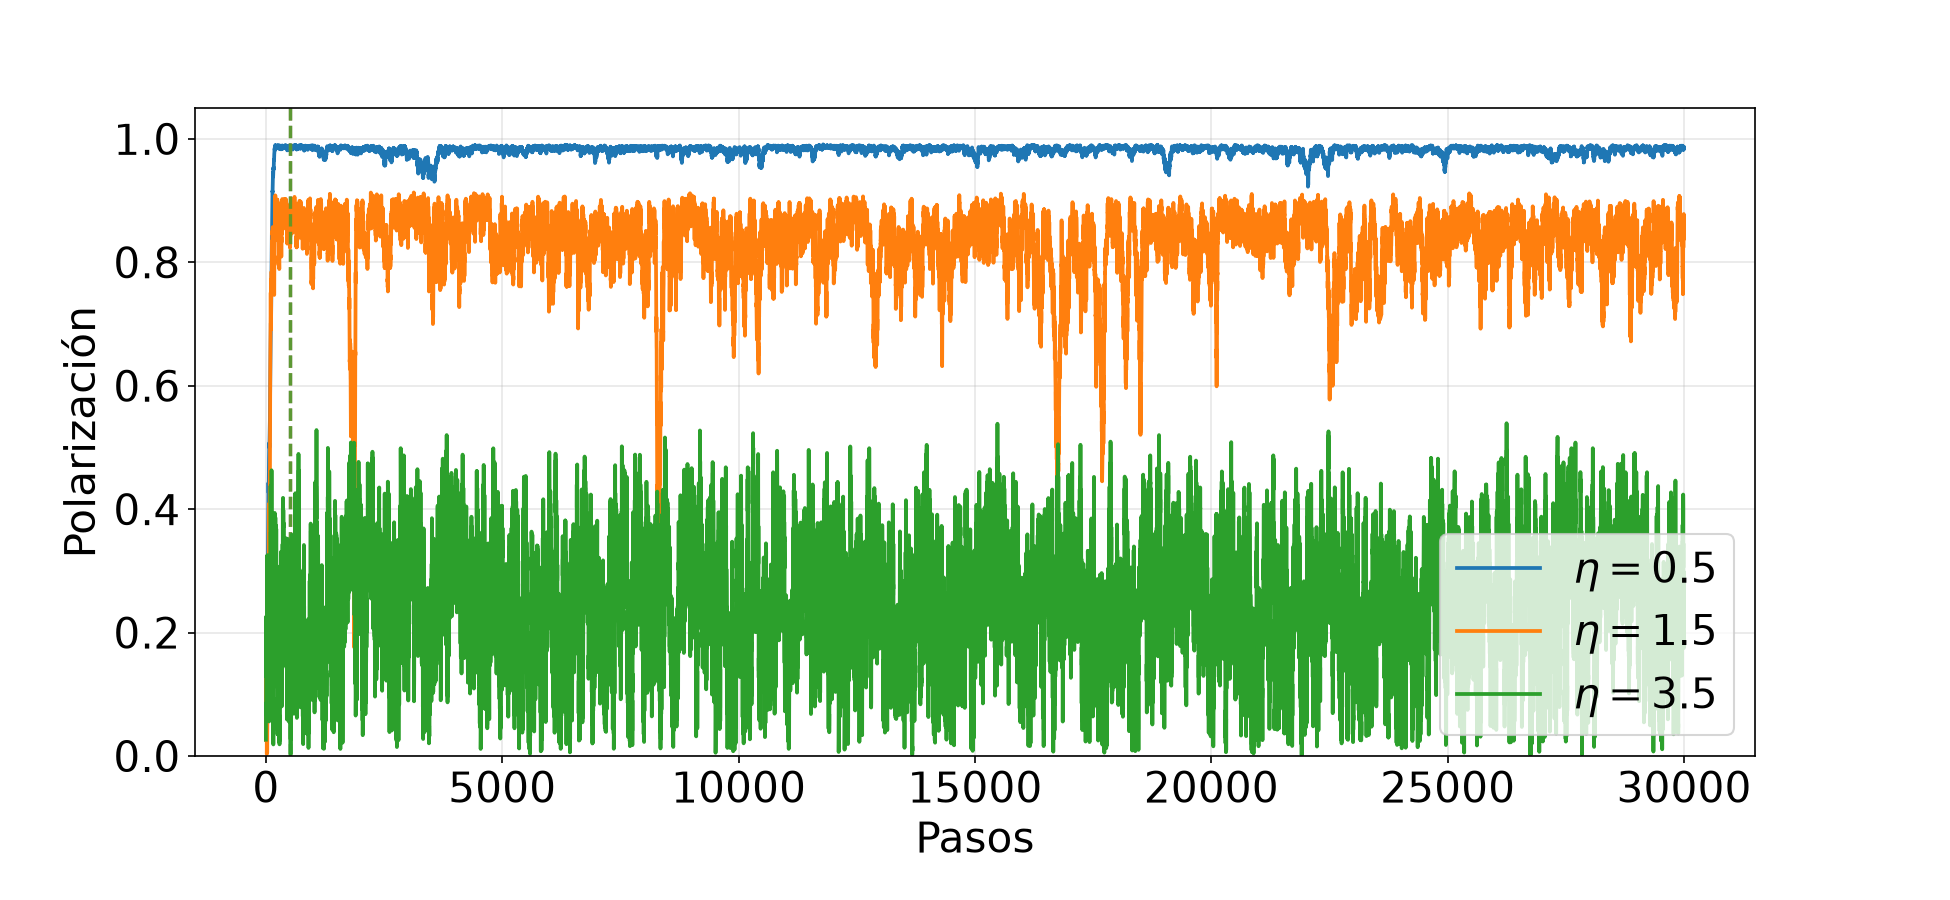
\includegraphics[width=0.8\textwidth]{entrega/b/evolucion_va_ruidos_30000_rho2.png}
  \caption{Evolución temporal de la polarización $v_a(t)$, modelo estándar,
    $\rho = 2$, para $\eta = 0.5,\ 1.5,\ 3.5$. Las líneas verticales
    punteadas indican $t_{\text{inicio}}$ de cada curva. $30\,000$ pasos.}
  \label{fig:b-standard-rho2}
\end{figure}

\begin{center}
  \fbox{\parbox{0.9\textwidth}{\centering\small
  Animación -- modelo de votante, $\rho = 2$, $\eta = 0.05$ y $0.5$:
  \href{https://youtu.be/XXXXX}{enlace pendiente}}}
\end{center}

La Fig.~\ref{fig:b-voter-rho2} muestra el mismo tipo de curva para el
modelo de votante con $\rho = 2$, para $\eta = 0.05$ y $\eta = 0.5$. Con
$\eta = 0.05$ el sistema se ordena de forma similar al caso estándar, con
$v_a$ cerca de $1$ y caídas transitorias ocasionales. Con $\eta = 0.5$ el
votante ya se encuentra en un régimen fuertemente desordenado, con $v_a$
oscilando de forma amplia entre $0$ y valores cercanos a $0.8$.

\begin{figure}[h]
  \centering
  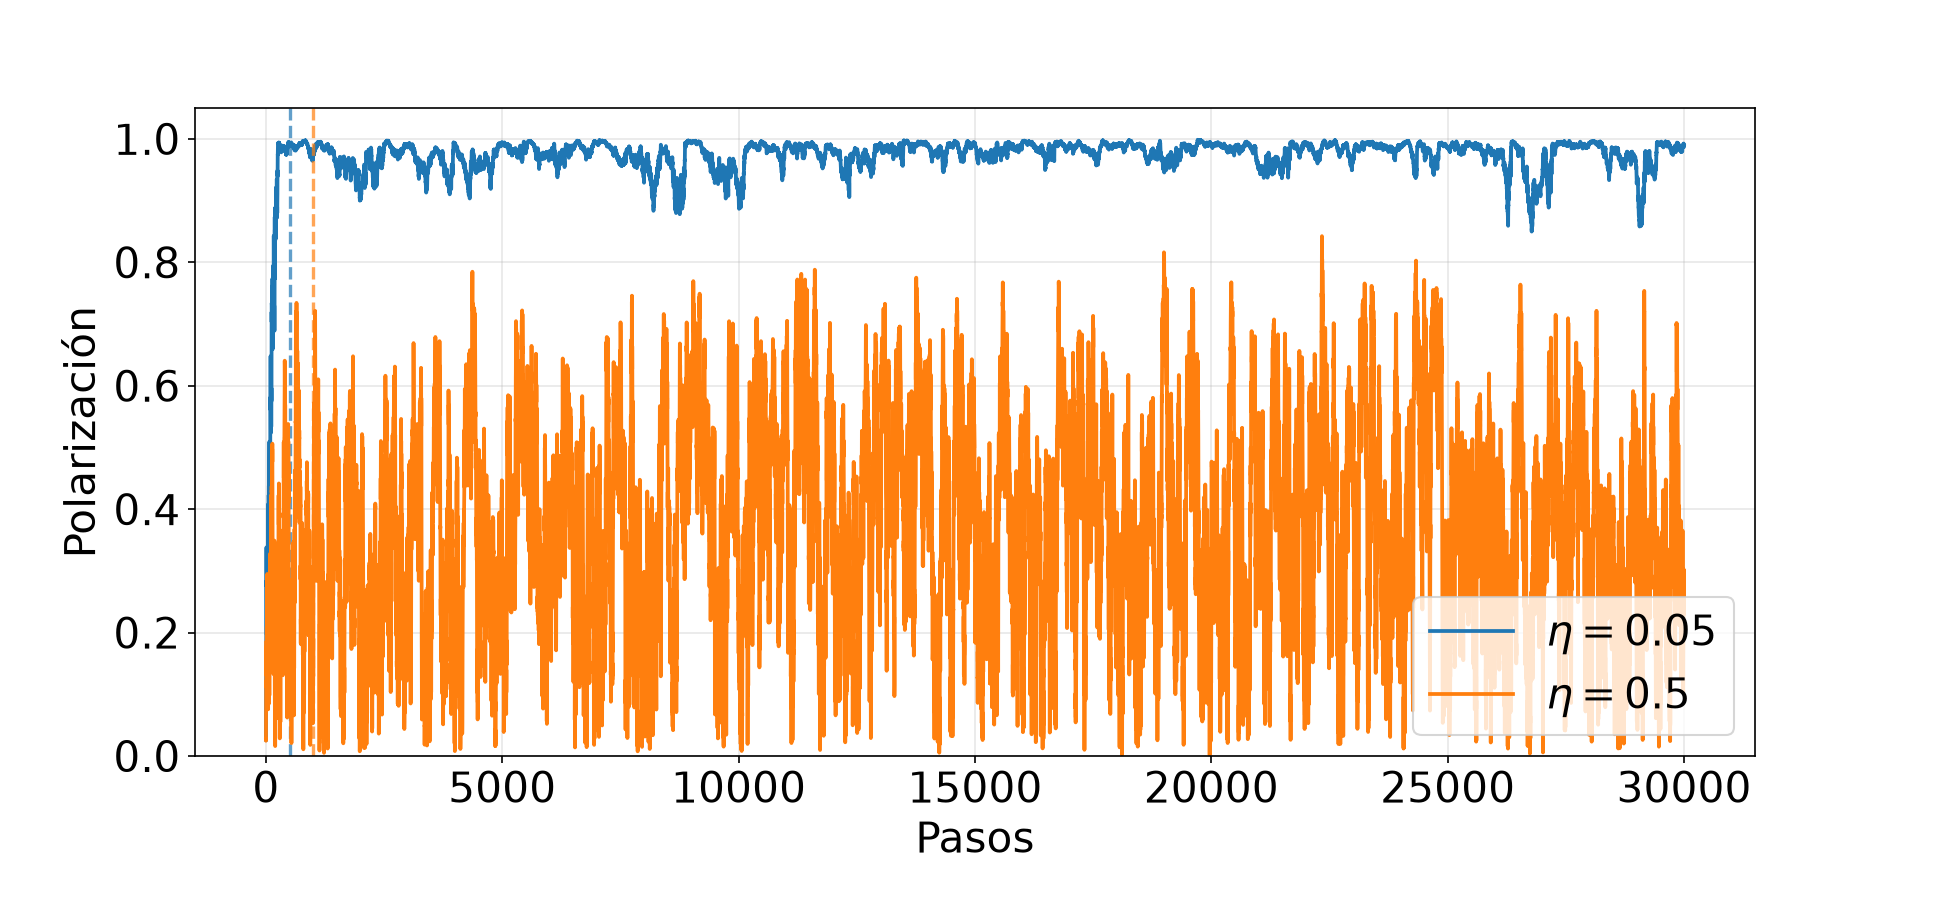
\includegraphics[width=0.8\textwidth]{entrega/b/evolucion_va_voter_30000_rho2.png}
  \caption{Evolución temporal de la polarización $v_a(t)$, modelo de
    votante, $\rho = 2$, para $\eta = 0.05,\ 0.5$. Las líneas verticales
    punteadas indican $t_{\text{inicio}}$ de cada curva. $30\,000$ pasos.}
  \label{fig:b-voter-rho2}
\end{figure}

\paragraph{Comparación estándar vs.\ votante ($\rho = 2$)}

Las Figs.~\ref{fig:b-standard-rho2} y \ref{fig:b-voter-rho2} muestran que, para
un mismo nivel de ruido ($\eta = 0.5$), el modelo estándar permanece en un
régimen ordenado y estable mientras que el votante ya está fuertemente
desordenado. Esto evidencia que el modelo de votante pierde el orden
colectivo con niveles de ruido mucho menores que el modelo estándar,
motivo por el cual se usó un rango de $\eta$ diez veces más chico para su
barrido.

\paragraph{$\rho = 4$}

\begin{center}
  \fbox{\parbox{0.9\textwidth}{\centering\small
  Animación -- modelo estándar, $\rho = 4$, $\eta = 0.5$ y $3.5$:
  \href{https://youtu.be/XXXXX}{enlace pendiente}}}
\end{center}

La Fig.~\ref{fig:b-standard} muestra la evolución temporal de $v_a(t)$ para
el modelo estándar con $\rho = 4$ y tres valores de ruido representativos.
Para $\eta = 0.5$, $v_a$ crece rápidamente hasta un valor cercano a $1$ y
permanece allí con fluctuaciones pequeñas durante toda la corrida: el
estado estacionario se alcanza casi de inmediato
($t_{\text{inicio}} = 500$). Para $\eta = 1.5$, la polarización se
estabiliza en torno a $0.85$--$0.9$ pero presenta caídas transitorias más
marcadas; se fijó $t_{\text{inicio}} = 8000$ para excluir un tramo inicial
en el que la amplitud de esas caídas era mayor. Para $\eta = 3.5$ el sistema
no alcanza un estado ordenado: $v_a$ fluctúa fuertemente en torno a un valor
medio bajo ($\approx 0.3$--$0.4$) desde el comienzo de la corrida, por lo
que $t_{\text{inicio}} = 500$ es suficiente.

\begin{figure}[h]
  \centering
  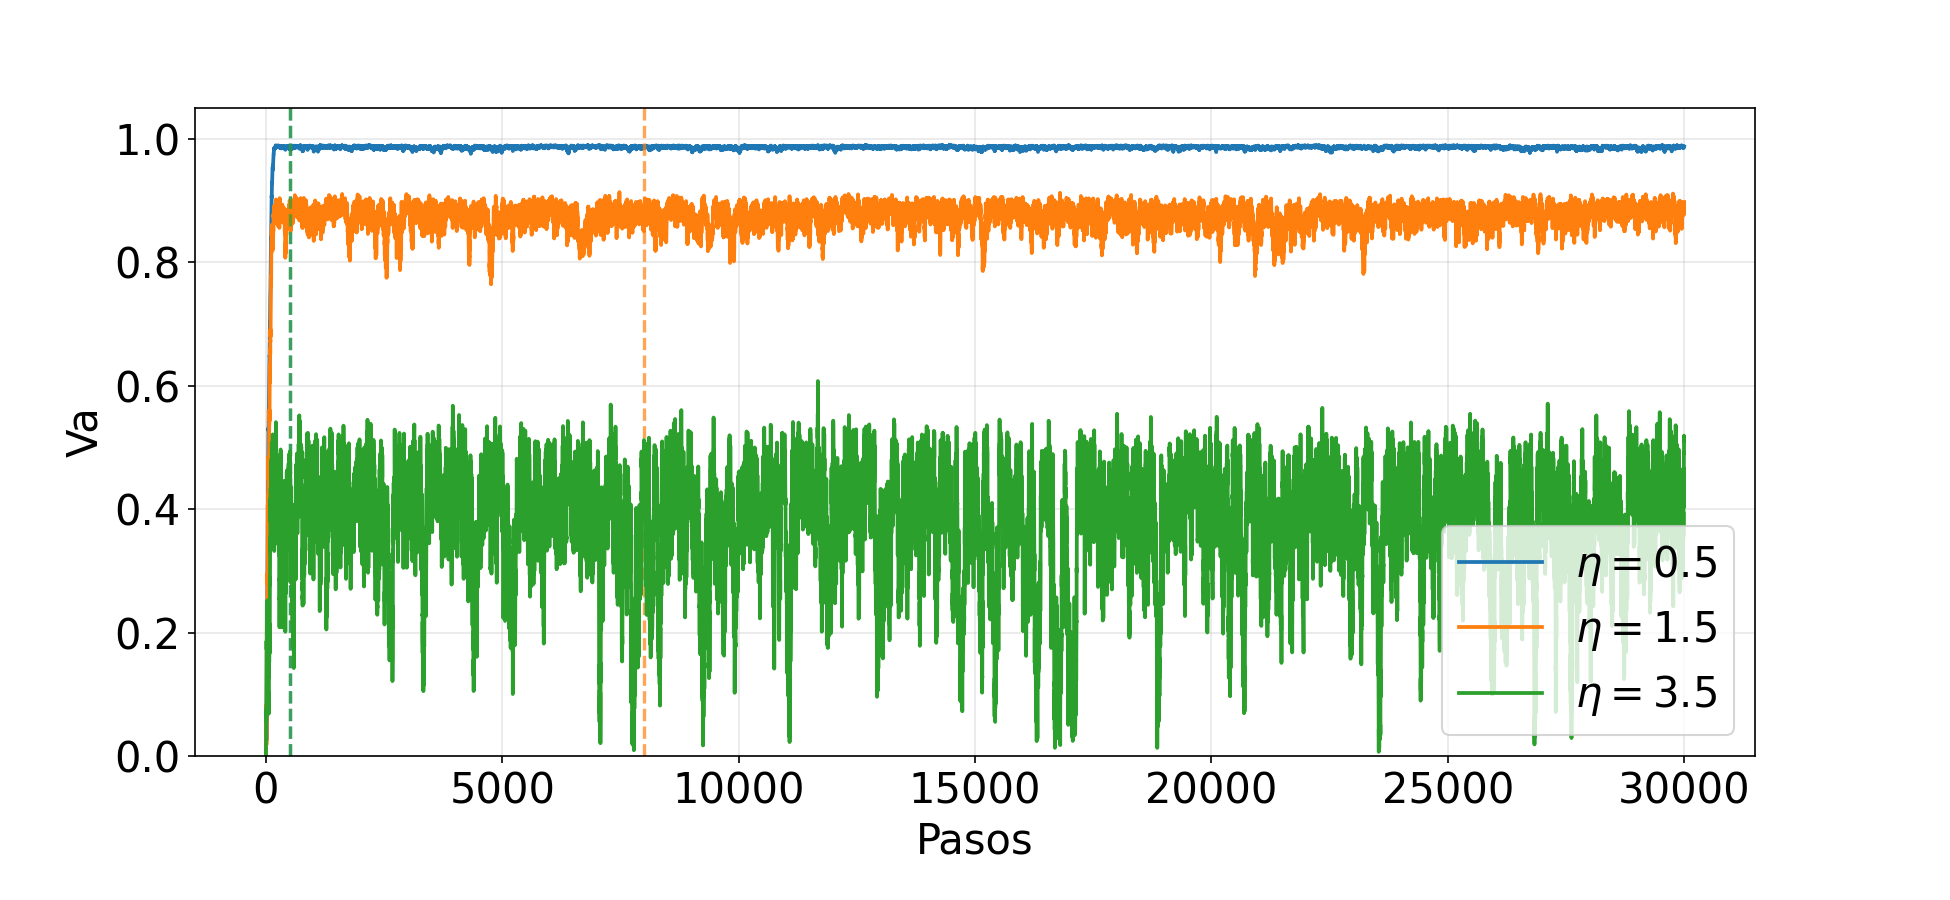
\includegraphics[width=0.8\textwidth]{entrega/b/evolucion_va_ruidos_30000.png}
  \caption{Evolución temporal de la polarización $v_a(t)$, modelo estándar,
    $\rho = 4$, para $\eta = 0.5,\ 1.5,\ 3.5$. Las líneas verticales
    punteadas indican $t_{\text{inicio}}$ de cada curva. $30\,000$ pasos.}
  \label{fig:b-standard}
\end{figure}

\begin{center}
  \fbox{\parbox{0.9\textwidth}{\centering\small
  Animación -- modelo de votante, $\rho = 4$, $\eta = 0.05$ y $0.5$:
  \href{https://youtu.be/XXXXX}{enlace pendiente}}}
\end{center}

La Fig.~\ref{fig:b-voter} muestra el mismo tipo de curva para el modelo de
votante, $\rho = 4$, con $\eta = 0.05$ y $\eta = 0.5$. Con $\eta = 0.05$
(ruido bajo dentro del rango del votante) el sistema se ordena de forma
similar al caso estándar, con $v_a$ cerca de $1$ y caídas transitorias
ocasionales. Con $\eta = 0.5$ -- un valor que en el modelo estándar todavía
corresponde a un régimen muy ordenado (Fig.~\ref{fig:b-standard}) -- el
modelo de votante ya se encuentra en un régimen fuertemente desordenado, con
$v_a$ oscilando de forma amplia entre $0$ y $0.7$.

\begin{figure}[h]
  \centering
  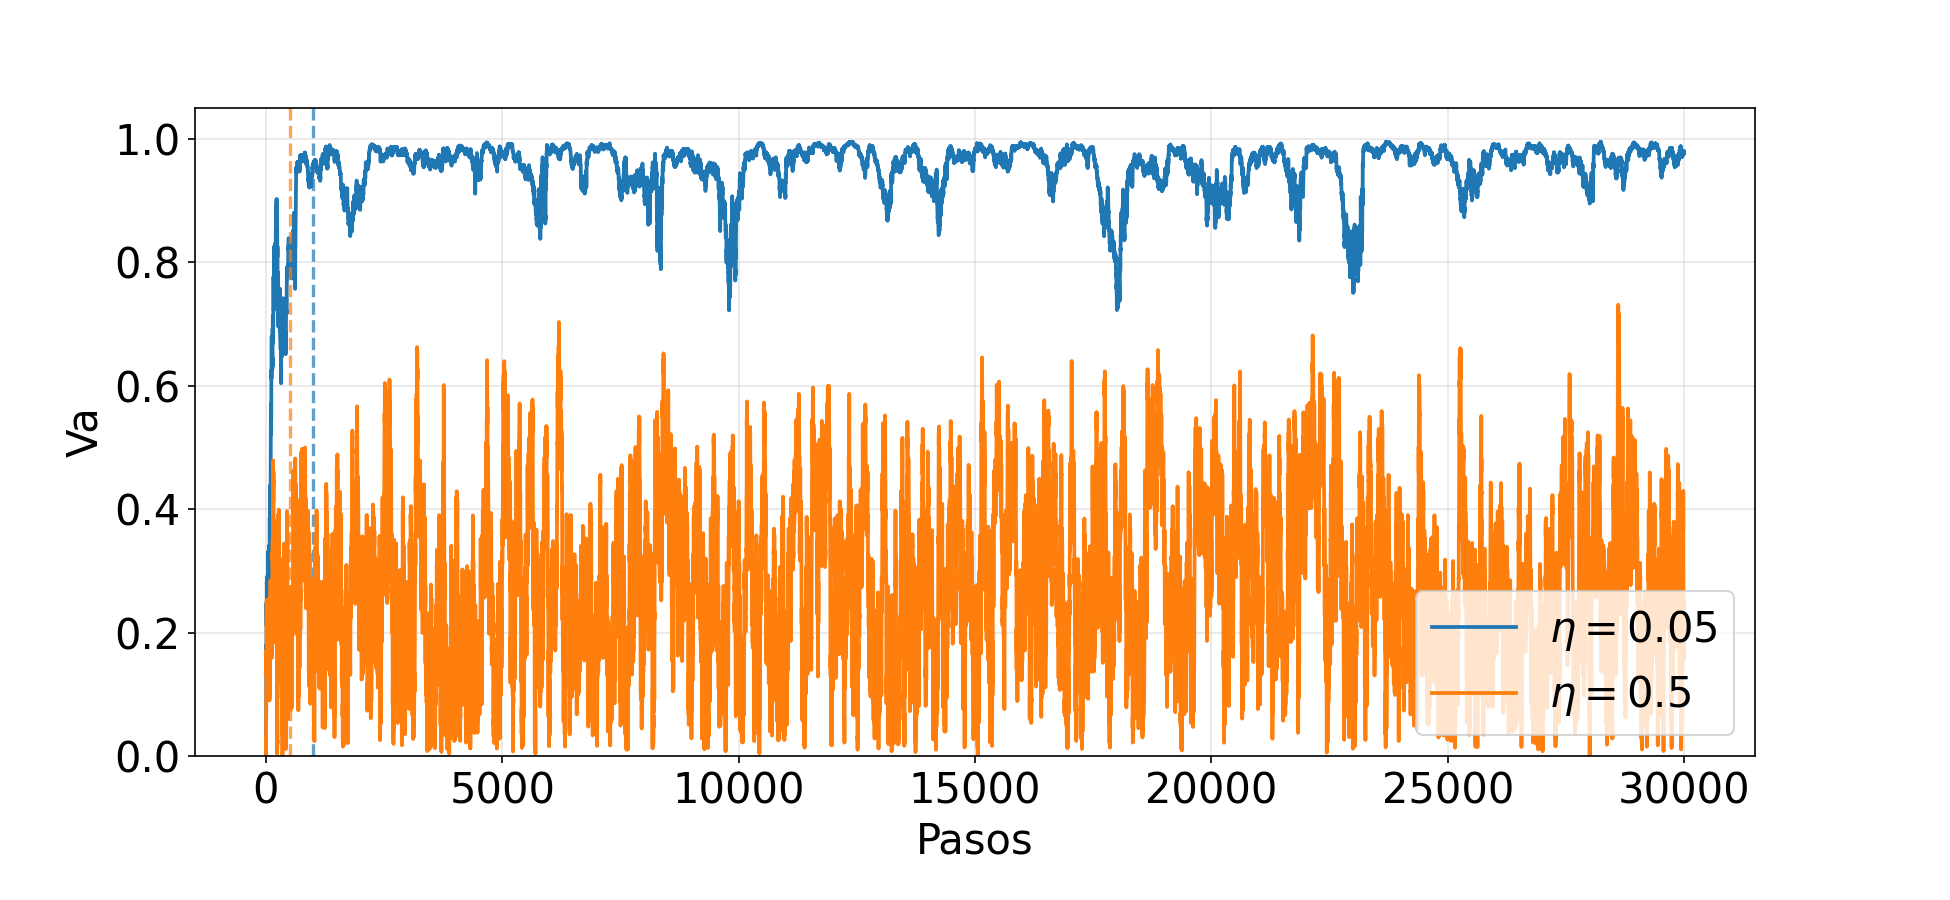
\includegraphics[width=0.8\textwidth]{entrega/b/evolucion_va_voter_30000.png}
  \caption{Evolución temporal de la polarización $v_a(t)$, modelo de
    votante, $\rho = 4$, para $\eta = 0.05,\ 0.5$. Las líneas verticales
    punteadas indican $t_{\text{inicio}}$ de cada curva. $30\,000$ pasos.}
  \label{fig:b-voter}
\end{figure}

\paragraph{Comparación estándar vs.\ votante ($\rho = 4$)}

Comparando las
Figs.~\ref{fig:b-standard} y \ref{fig:b-voter} se confirma el mismo patrón
que a $\rho = 2$: un $\eta$ que en el modelo estándar corresponde a un
régimen muy ordenado deja al votante fuertemente desordenado. Esto es
consistente con la regla de actualización de cada modelo: mientras Vicsek
promedia sobre todos los vecinos (Ec.~\eqref{eq:vicsek}), lo que atenúa el
efecto del ruido individual de cada vecino, el votante copia la dirección
de un único vecino (Ec.~\eqref{eq:voter}), heredando además todo el ruido
acumulado por ese vecino en el paso anterior, lo que hace al sistema mucho
más sensible a $\eta$.

\paragraph{$\rho = 8$}

\begin{center}
  \fbox{\parbox{0.9\textwidth}{\centering\small
  Animación -- modelo estándar, $\rho = 8$, $\eta = 0.5$ y $3.5$:
  \href{https://youtu.be/XXXXX}{enlace pendiente}}}
\end{center}

La Fig.~\ref{fig:b-standard-rho8} muestra la evolución temporal de
$v_a(t)$ para el modelo estándar con $\rho = 8$. El patrón cualitativo es
el mismo que a $\rho = 2$ y $\rho = 4$, pero mucho más estable: con
$\eta = 0.5$, $v_a$ permanece casi constante en $\approx 0.99$; con
$\eta = 1.5$, las caídas transitorias del régimen intermedio son pequeñas y
poco frecuentes (a diferencia de las caídas marcadas de $\rho = 2$); y con
$\eta = 3.5$ el sistema fluctúa en el régimen desordenado en torno a un
valor medio más alto ($\approx 0.45$--$0.55$) que a densidades menores.
Esto es consistente con el efecto de la densidad: más vecinos por
partícula hacen que el promedio angular de la Ec.~\eqref{eq:vicsek} sea
más robusto frente al ruido individual.

\begin{figure}[h]
  \centering
  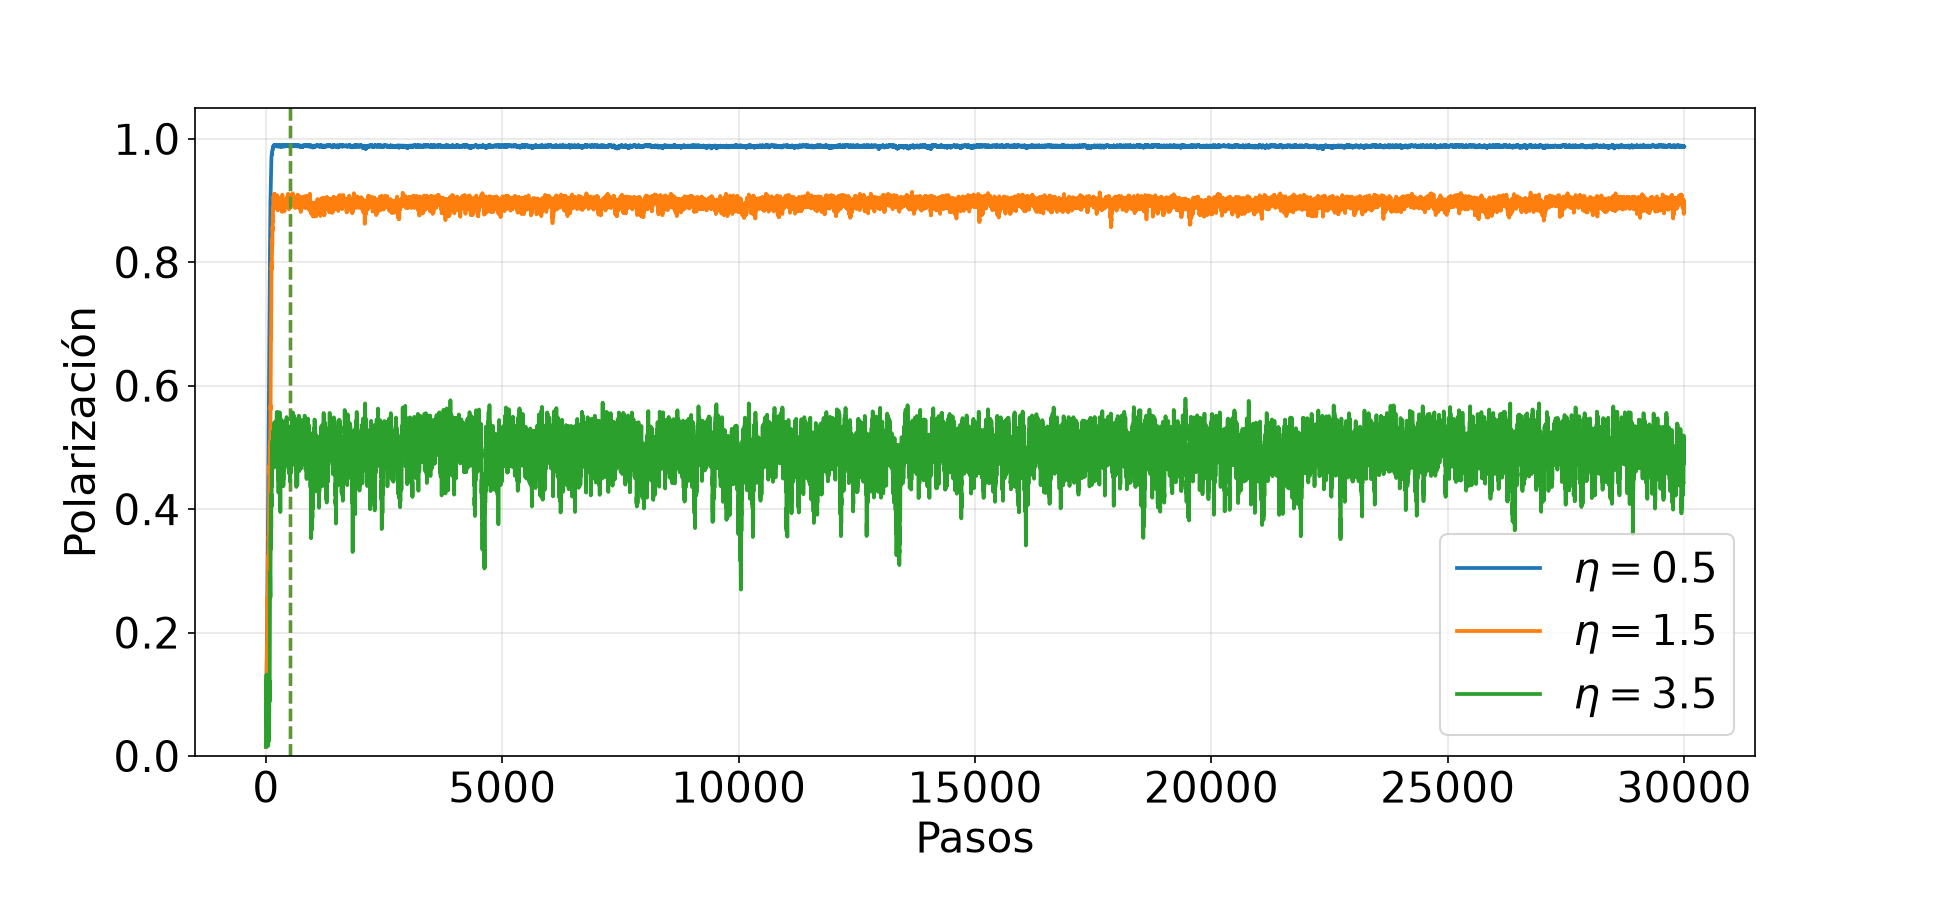
\includegraphics[width=0.8\textwidth]{entrega/b/evolucion_va_ruidos_30000_rho8.png}
  \caption{Evolución temporal de la polarización $v_a(t)$, modelo estándar,
    $\rho = 8$, para $\eta = 0.5,\ 1.5,\ 3.5$. Las líneas verticales
    punteadas indican $t_{\text{inicio}}$ de cada curva. $30\,000$ pasos.}
  \label{fig:b-standard-rho8}
\end{figure}

\begin{center}
  \fbox{\parbox{0.9\textwidth}{\centering\small
  Animación -- modelo de votante, $\rho = 8$, $\eta = 0.05$ y $0.5$:
  \href{https://youtu.be/XXXXX}{enlace pendiente}}}
\end{center}

La Fig.~\ref{fig:b-voter-rho8} muestra el mismo estudio para el modelo de
votante con $\rho = 8$, y aparece una diferencia cualitativa respecto de
$\rho = 2$ y $\rho = 4$: con $\eta = 0.05$ el sistema tarda notoriamente
más en alcanzar el estado estacionario (más de $3000$ pasos, frente a los
menos de $500$ que demoran $\rho = 2$ y $\rho = 4$) y, una vez alcanzado,
sigue mostrando caídas transitorias profundas y recurrentes. Con
$\eta = 0.5$, $v_a$ fluctúa entre $0$ y valores algo menores que a
$\rho = 2$.

\begin{figure}[h]
  \centering
  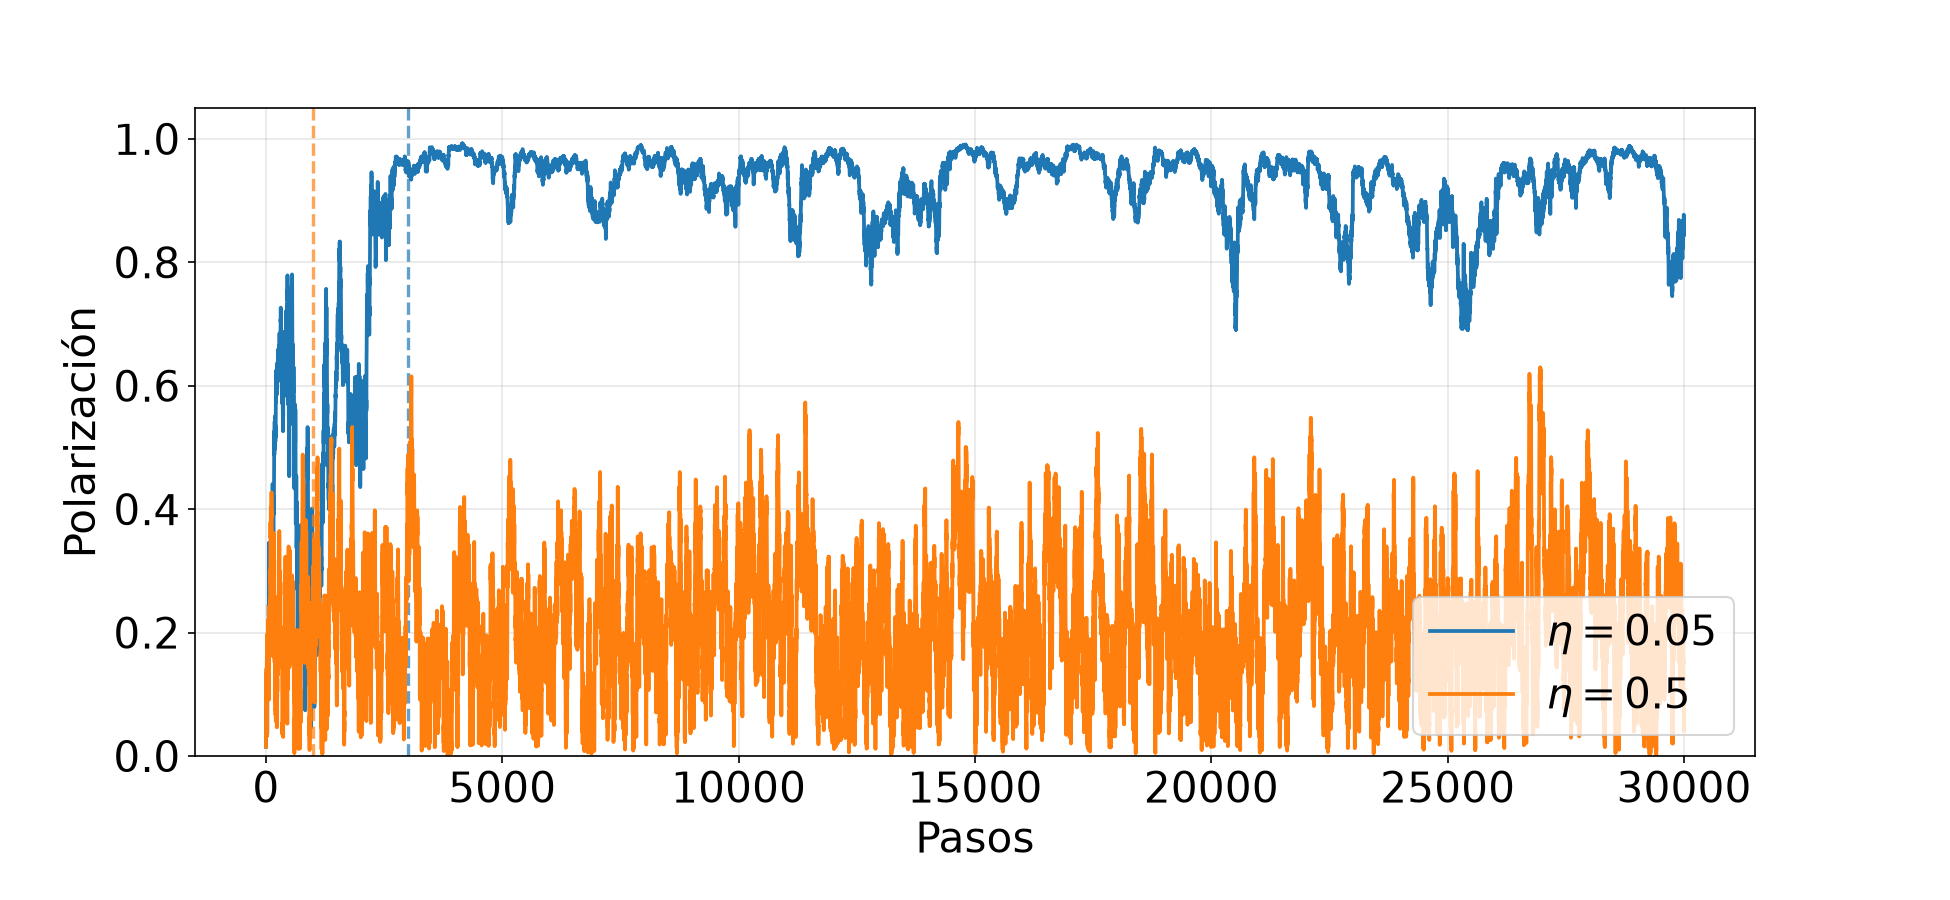
\includegraphics[width=0.8\textwidth]{entrega/b/evolucion_va_voter_30000_rho8.png}
  \caption{Evolución temporal de la polarización $v_a(t)$, modelo de
    votante, $\rho = 8$, para $\eta = 0.05,\ 0.5$. Las líneas verticales
    punteadas indican $t_{\text{inicio}}$ de cada curva. $30\,000$ pasos.}
  \label{fig:b-voter-rho8}
\end{figure}

\paragraph{Comparación estándar vs.\ votante ($\rho = 8$)}

A diferencia de lo
que ocurre en el modelo estándar, donde $\rho = 8$ es siempre la densidad
más estable (Fig.~\ref{fig:b-standard-rho8}), el votante con $\rho = 8$ y
ruido bajo (Fig.~\ref{fig:b-voter-rho8}) tarda más en alcanzar el estado
estacionario y sigue mostrando caídas transitorias profundas. Esto sugiere
que, al copiar la dirección de un único vecino en lugar de promediar, una
densidad alta no estabiliza al modelo de votante de la misma forma
sistemática que al estándar: en poblaciones grandes, dominios de
partículas pueden copiarse direcciones incorrectas entre sí de forma
correlacionada, produciendo caídas colectivas de $v_a$ incluso en el
régimen de ruido bajo.

\subsubsection{Polarización media en función del ruido}

\paragraph{Densidades altas ($\rho = 2, 4, 8$)}

\begin{center}
  \fbox{\parbox{0.9\textwidth}{\centering\small
  Animación -- modelo estándar, $\rho = 2, 4, 8$, $\eta = 0$ y $5$:
  \href{https://youtu.be/XXXXX}{enlace pendiente}}}
\end{center}

La Fig.~\ref{fig:c-standard-high} muestra $\langle v_a \rangle \pm
\sigma_{v_a}$ en función de $\eta$ para el modelo estándar con las tres
densidades altas ($\rho = 2, 4, 8$). En los tres casos
se observa una transición continua desde un estado ordenado
($v_a \approx 1$ para $\eta$ chico) hacia uno desordenado
($v_a \lesssim 0.1$ para $\eta$ cercano a $5$), con la caída más pronunciada
en el rango $\eta \in [2, 4]$. A igual $\eta$, la densidad más alta
($\rho = 8$) sostiene un valor de $v_a$ mayor que las densidades más bajas
en todo el rango intermedio: a mayor densidad, cada partícula tiene en
promedio más vecinos, por lo que el promedio de la Ec.~\eqref{eq:vicsek} se
calcula sobre más términos y resulta más robusto frente al ruido individual
de cada partícula.

\begin{figure}[h]
  \centering
  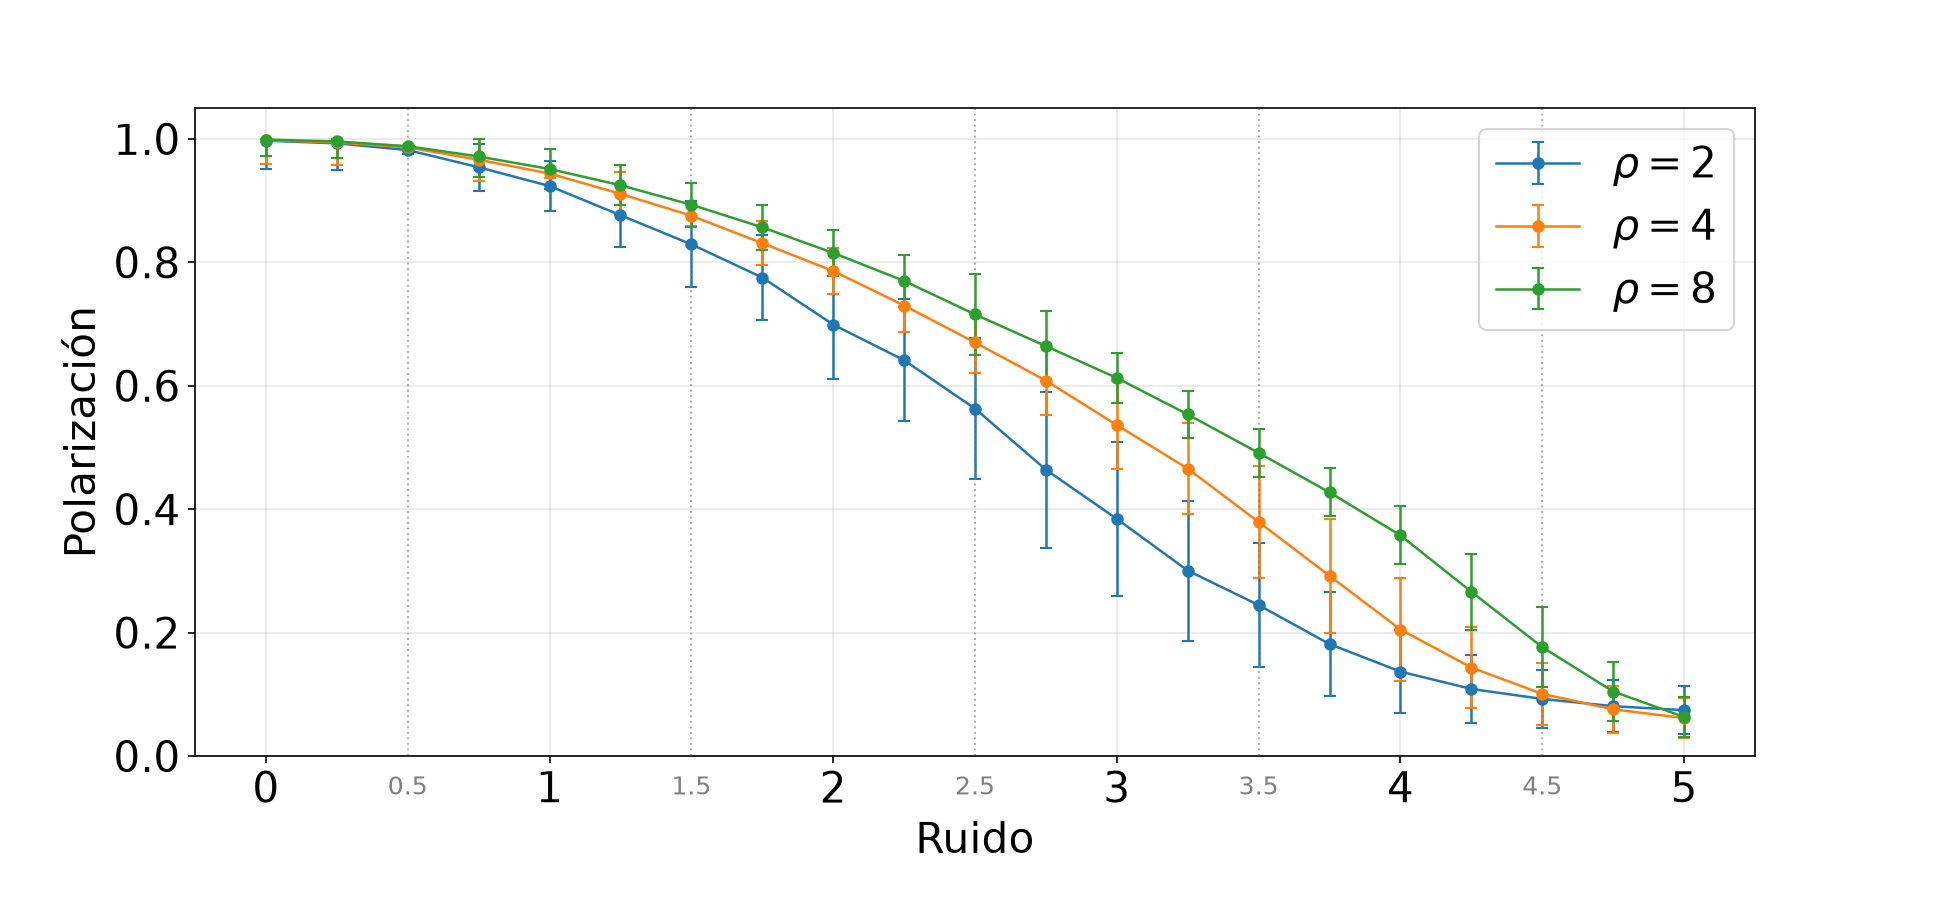
\includegraphics[width=0.75\textwidth]{entrega/c/c_standard_3dens_30000.png}
  \caption{Polarización media $\langle v_a \rangle \pm \sigma_{v_a}$ en
    función del ruido $\eta$, modelo estándar, para $\rho = 2, 4, 8$.
    $30\,000$ pasos.}
  \label{fig:c-standard-high}
\end{figure}

\begin{center}
  \fbox{\parbox{0.9\textwidth}{\centering\small
  Animación -- modelo de votante, $\rho = 2, 4, 8$, $\eta = 0$ y $1$:
  \href{https://youtu.be/XXXXX}{enlace pendiente}}}
\end{center}

La Fig.~\ref{fig:c-voter-high} muestra el mismo análisis para el modelo de
votante con $\rho = 2, 4, 8$: una transición cualitativamente similar a la
del modelo estándar -- mayor densidad sostiene mayor $v_a$ a igual $\eta$
-- pero comprimida en un rango de ruido diez veces menor, y con un valor
residual de $v_a$ que no decae por debajo de $\approx 0.15$--$0.2$ incluso
en $\eta = 1$, a diferencia del modelo estándar que sigue decreciendo hasta
$\eta = 5$.

\begin{figure}[h]
  \centering
  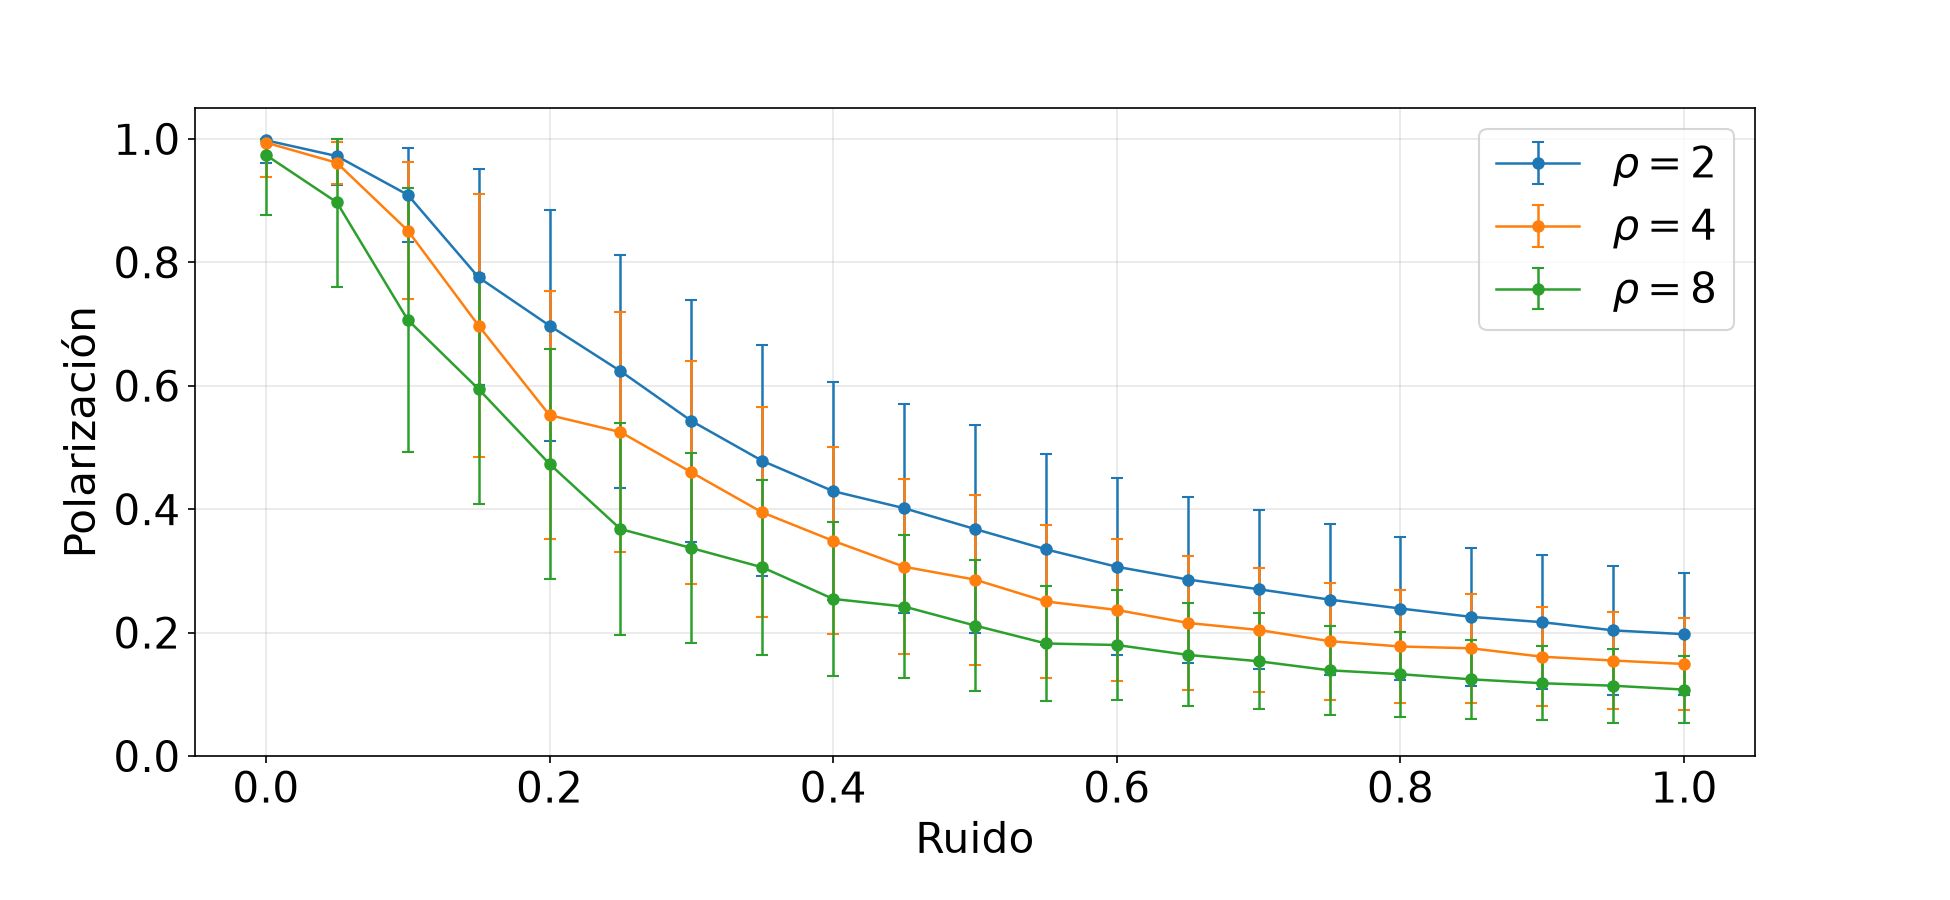
\includegraphics[width=0.75\textwidth]{entrega/c/c_voter_3dens_30000.png}
  \caption{Polarización media $\langle v_a \rangle \pm \sigma_{v_a}$ en
    función del ruido $\eta$, modelo de votante, para $\rho = 2, 4, 8$.
    $30\,000$ pasos.}
  \label{fig:c-voter-high}
\end{figure}

\paragraph{Comparación estándar vs.\ votante (densidades altas)}

La
diferencia principal entre ambos modelos en las Figs.~\ref{fig:c-standard-high}
y \ref{fig:c-voter-high} no es cualitativa sino de escala: ambos muestran
una transición continua de un estado ordenado a uno desordenado gobernada
por $\eta$, y en ambos la densidad favorece el orden. La diferencia
central es que el modelo de votante pierde el orden colectivo con una
amplitud de ruido casi un orden de magnitud menor que el modelo estándar,
consistente con lo observado en las curvas temporales de la sección
anterior.

\paragraph{Densidades bajas}

\begin{center}
  \fbox{\parbox{0.9\textwidth}{\centering\small
  Animación -- modelo estándar, $\rho = 1/\pi, 1/(2\pi), 1/(3\pi)$,
  $\eta = 0$ y $5$: \href{https://youtu.be/XXXXX}{enlace pendiente}}}
\end{center}

La Fig.~\ref{fig:c-standard-low} repite el mismo estudio para las tres
densidades bajas ($\rho = 1/\pi, 1/(2\pi), 1/(3\pi)$). A diferencia del caso
anterior, las tres curvas son indistinguibles entre sí dentro de las barras
de error en prácticamente todo el rango de $\eta$: con $N$ tan chico
($10$--$31$ partículas), la cantidad de vecinos promedio ya es baja para las
tres densidades, y reducirla aún más no introduce una diferencia
apreciable en $v_a$. Las barras de error también son notablemente más
grandes que en la Fig.~\ref{fig:c-standard-high}, reflejo de la mayor
fluctuación estadística asociada a un $N$ chico.

\begin{figure}[h]
  \centering
  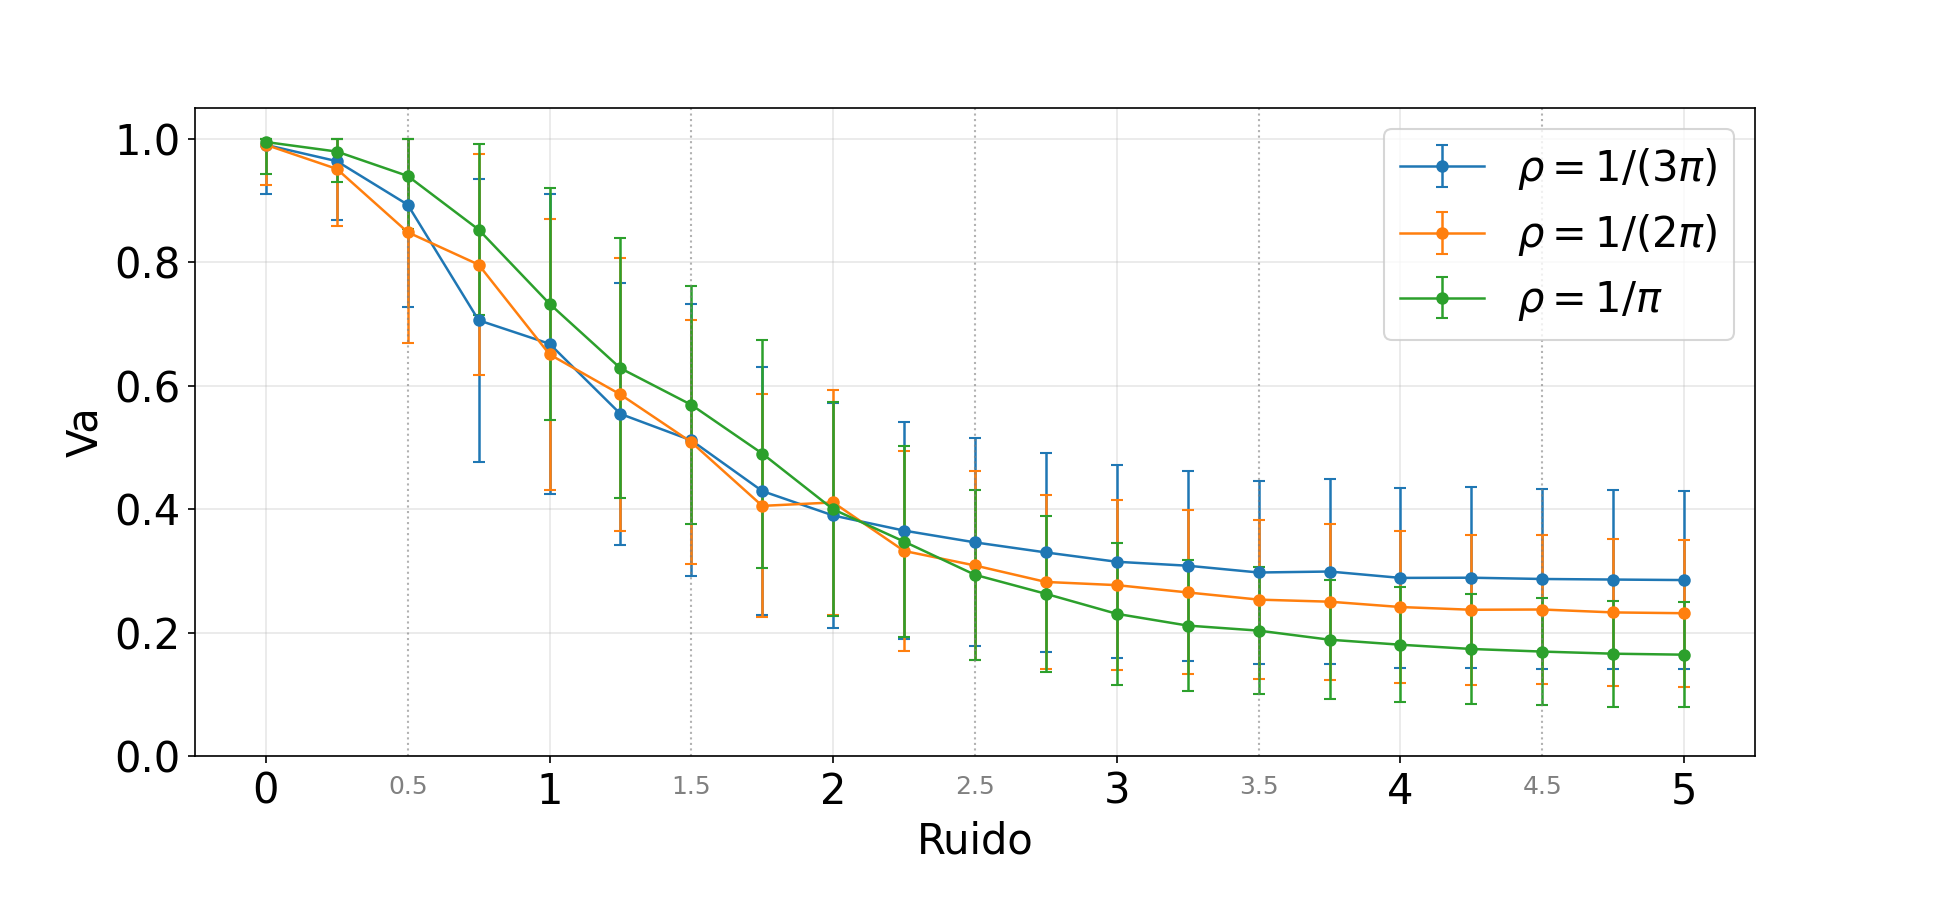
\includegraphics[width=0.75\textwidth]{entrega/c/c_standard_lowdens_30000.png}
  \caption{Polarización media $\langle v_a \rangle \pm \sigma_{v_a}$ en
    función del ruido $\eta$, modelo estándar, para
    $\rho = 1/\pi,\ 1/(2\pi),\ 1/(3\pi)$. $30\,000$ pasos.}
  \label{fig:c-standard-low}
\end{figure}

\begin{center}
  \fbox{\parbox{0.9\textwidth}{\centering\small
  Animación -- modelo de votante, $\rho = 1/\pi, 1/(3\pi)$, $\eta = 0$ y
  $1$: \href{https://youtu.be/XXXXX}{enlace pendiente}}}
\end{center}

La Fig.~\ref{fig:c-voter-low} muestra el mismo estudio para el modelo de
votante, igual que en el caso estándar con curvas superpuestas dentro del
error y fluctuaciones no monótonas producto del $N$ chico; siguiendo la
nota de la Sección~\ref{sec:resultados}, esta figura sólo incluye
$\rho = 1/\pi$ y $\rho = 1/(3\pi)$.

\begin{figure}[h]
  \centering
  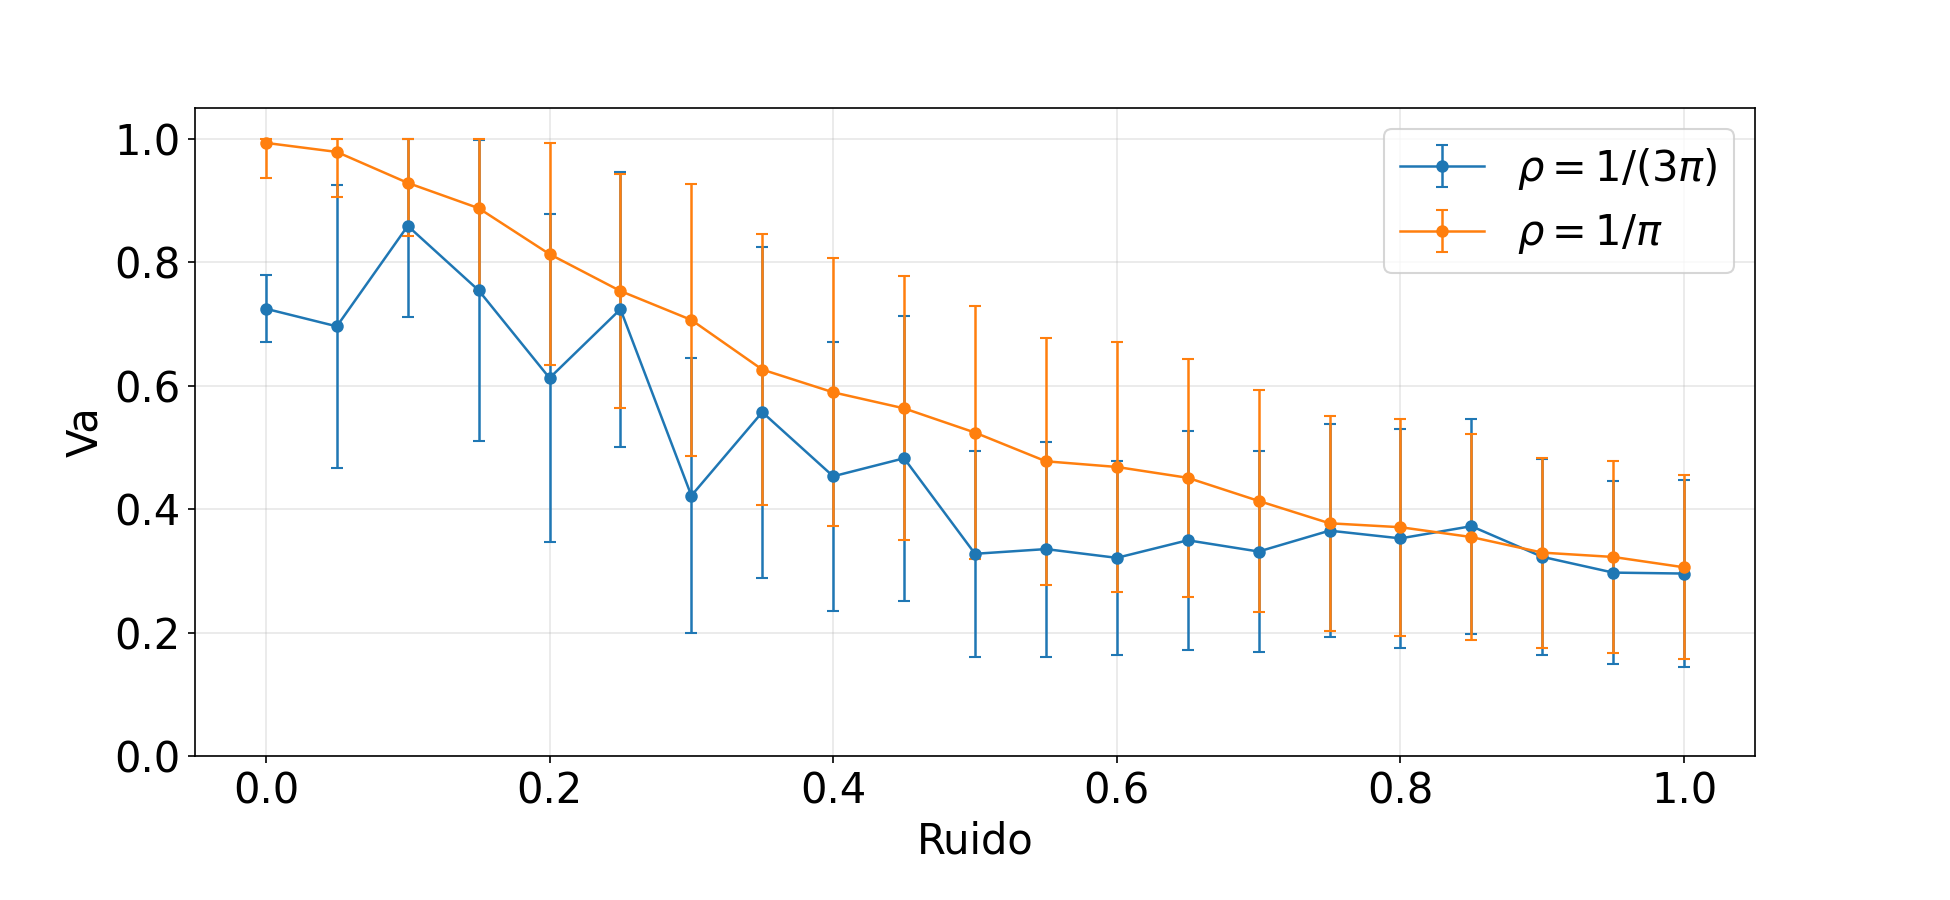
\includegraphics[width=0.75\textwidth]{entrega/c/c_voter_lowdens_30000.png}
  \caption{Polarización media $\langle v_a \rangle \pm \sigma_{v_a}$ en
    función del ruido $\eta$, modelo de votante, para
    $\rho = 1/\pi,\ 1/(3\pi)$. $30\,000$ pasos.}
  \label{fig:c-voter-low}
\end{figure}

\paragraph{Comparación estándar vs.\ votante (densidades bajas)}

Las
Figs.~\ref{fig:c-standard-low} y \ref{fig:c-voter-low} muestran el mismo
comportamiento en ambos modelos: con $N$ tan chico, el efecto de la
densidad sobre $v_a$ desaparece y las curvas quedan dominadas por
fluctuación estadística antes que por la regla de actualización angular.
La diferencia de escala en $\eta$ entre modelos se mantiene, pero ya no se
observa el ordenamiento por densidad que sí aparece a densidades altas.

\subsection{Clusters}

Para estudiar el rol de la conectividad espacial se comparó, para cada
modelo, la densidad $\rho = 2$ con la densidad baja $\rho = 1/\pi$, a un
$\eta$ fijo representativo de cada modelo ($\eta = 0.5$ para el estándar,
$\eta = 0.1$ para el votante).

\paragraph{Evolución temporal de $S$}

\begin{center}
  \fbox{\parbox{0.9\textwidth}{\centering\small
  Animación -- modelo estándar, $\rho = 2$ y $1/\pi$, $\eta = 0.5$:
  \href{https://youtu.be/XXXXX}{enlace pendiente}}}
\end{center}

La Fig.~\ref{fig:d1-standard} muestra $S(t)$ para el modelo estándar. Con
$\rho = 2$ ($N = 200$), $S$ permanece prácticamente en $1$ durante toda la
corrida: a esa densidad, la red de vecindad definida por $r_c$ está muy por
encima del umbral de percolación geométrica y casi todas las partículas
pertenecen a un único cluster en todo momento. Con $\rho = 1/\pi$
($N = 31$), en cambio, $S$ fluctúa de forma marcada entre valores cercanos a
$1$ y caídas por debajo de $0.5$: a esa densidad el sistema está cerca del
umbral de percolación, por lo que pequeños cambios en la configuración
espacial alcanzan para fragmentar o reconectar el cluster más grande.

\begin{figure}[h]
  \centering
  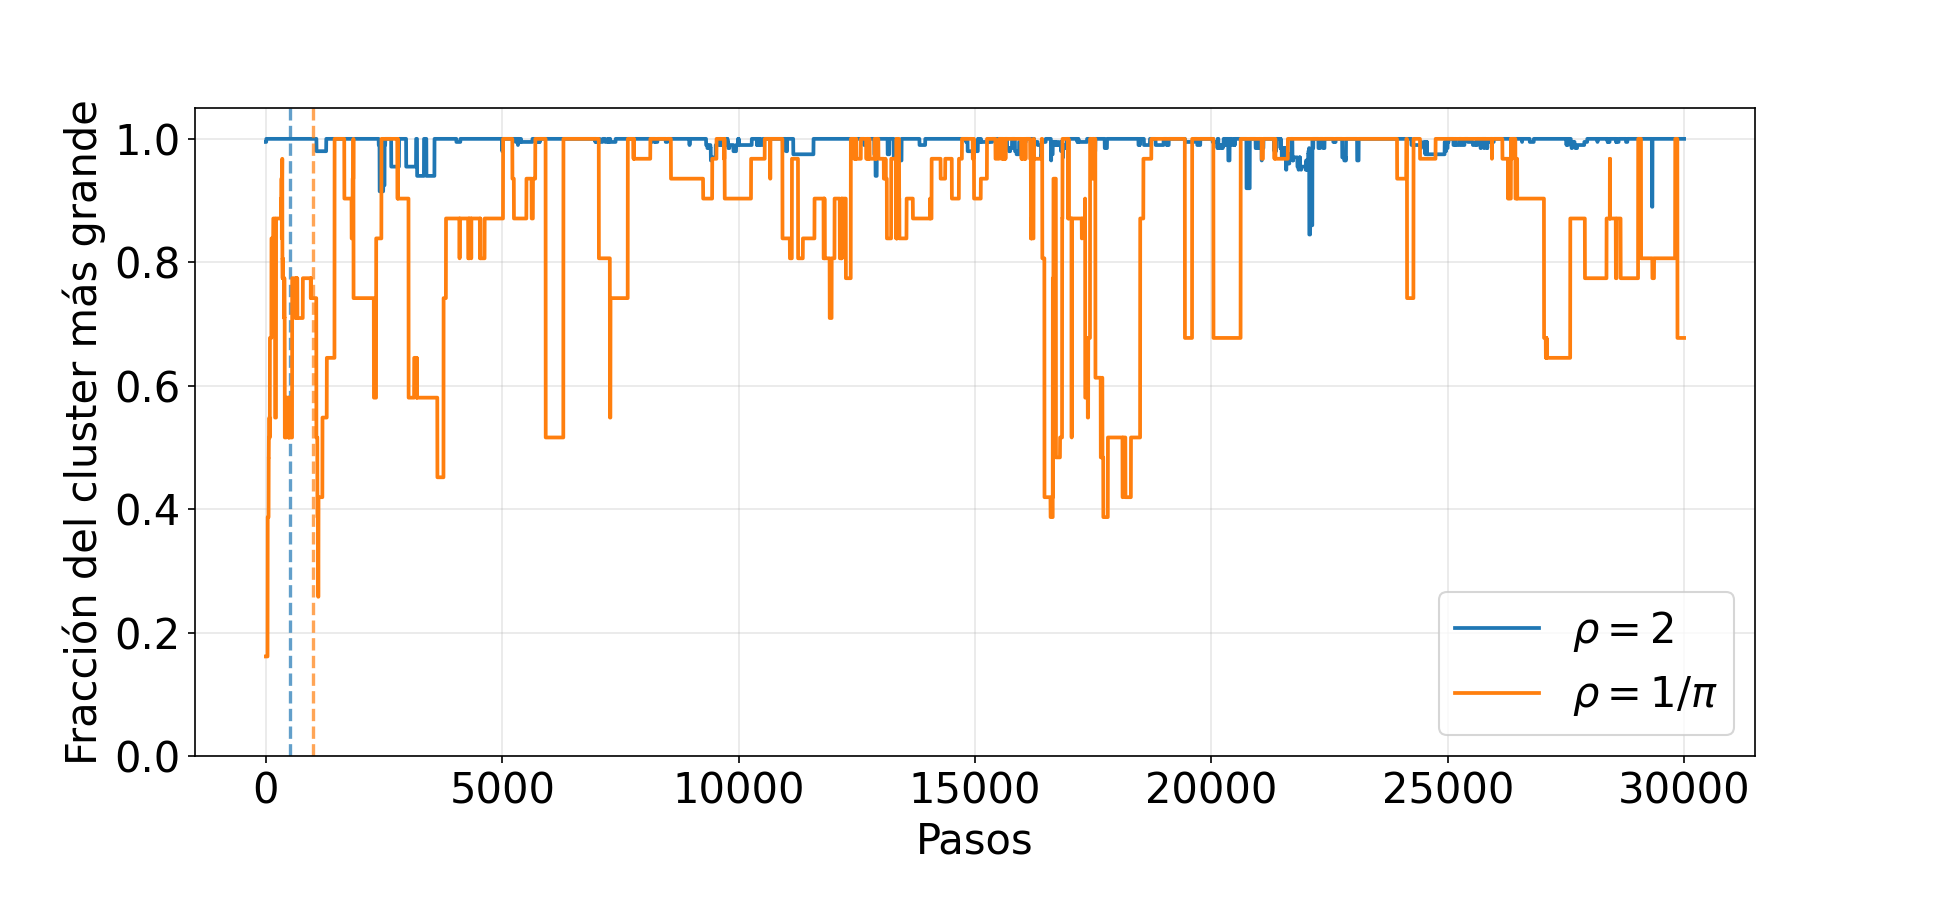
\includegraphics[width=0.8\textwidth]{entrega/d1/d1_standard_2_vs_low_30000.png}
  \caption{Evolución temporal de la fracción del cluster más grande $S(t)$,
    modelo estándar, $\eta = 0.5$, para $\rho = 2$ y $\rho = 1/\pi$. Las
    líneas verticales punteadas indican $t_{\text{inicio}}$ de cada curva.
    $30\,000$ pasos.}
  \label{fig:d1-standard}
\end{figure}

\begin{center}
  \fbox{\parbox{0.9\textwidth}{\centering\small
  Animación -- modelo de votante, $\rho = 2$ y $1/\pi$, $\eta = 0.1$:
  \href{https://youtu.be/XXXXX}{enlace pendiente}}}
\end{center}

La Fig.~\ref{fig:d1-voter} muestra el mismo estudio para el modelo de
votante: con $\rho = 2$ el valor de $S$ se mantiene cerca de $1$ y con
$\rho = 1/\pi$ fluctúa fuertemente cerca del umbral de percolación, igual
que en el modelo estándar.

\begin{figure}[h]
  \centering
  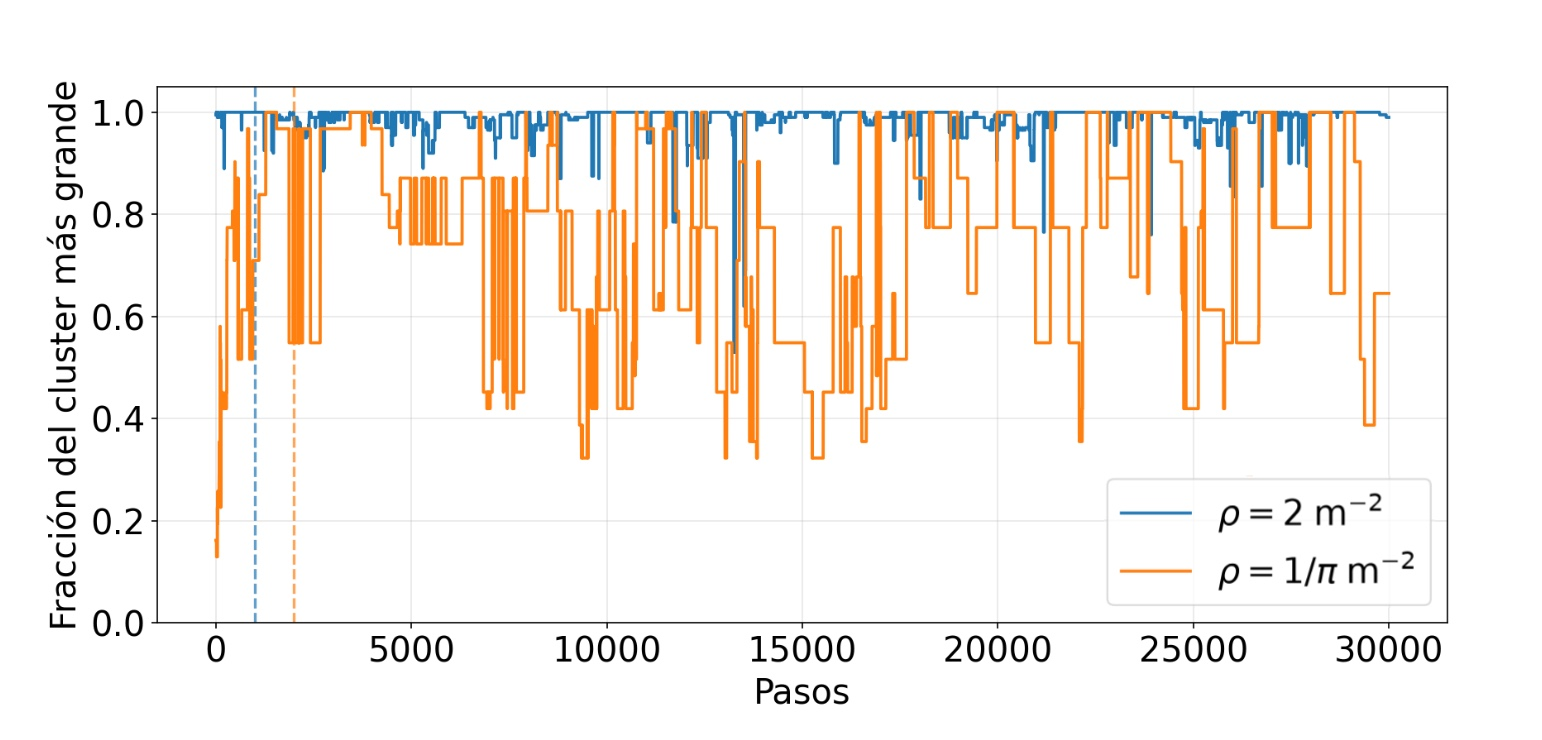
\includegraphics[width=0.8\textwidth]{entrega/d1/d1_voter_2_vs_low_30000.png}
  \caption{Evolución temporal de la fracción del cluster más grande $S(t)$,
    modelo de votante, $\eta = 0.1$, para $\rho = 2$ y $\rho = 1/\pi$. Las
    líneas verticales punteadas indican $t_{\text{inicio}}$ de cada curva.
    $30\,000$ pasos.}
  \label{fig:d1-voter}
\end{figure}

\paragraph{Comparación estándar vs.\ votante ($S(t)$)}

El comportamiento
cualitativo de las Figs.~\ref{fig:d1-standard} y \ref{fig:d1-voter} es el
mismo en ambos modelos -- $\rho = 2$ se mantiene cerca de $S = 1$ y
$\rho = 1/\pi$ fluctúa fuertemente cerca del umbral de percolación --
aunque en el votante $\rho = 2$ presenta caídas transitorias algo más
profundas (hasta $\approx 0.3$) que en el modelo estándar. Esto es
consistente con que $S$ depende de las posiciones, que en ambos modelos se
actualizan de la misma forma (Ec.~\eqref{eq:posicion}), y no directamente
de la regla angular que sí distingue a los dos modelos.

\paragraph{Fracción media del cluster más grande vs.\ ruido}

\begin{center}
  \fbox{\parbox{0.9\textwidth}{\centering\small
  Animación -- modelo estándar, $\rho = 2$ y $1/\pi$, $\eta = 0$ y $5$:
  \href{https://youtu.be/XXXXX}{enlace pendiente}}}
\end{center}

La Fig.~\ref{fig:d2-standard} muestra $\langle S \rangle \pm \sigma_S$ en
función de $\eta$ para el modelo estándar, siguiendo el mismo
procedimiento de estado estacionario usado para $v_a$. Con $\rho = 2$,
$\langle S \rangle \approx 0.95$--$1$ se mantiene prácticamente constante
en todo el rango de $\eta$: al estar muy por encima del umbral de
percolación, la conectividad espacial no depende del nivel de ruido. Con
$\rho = 1/\pi$, en cambio, $\langle S \rangle$ decrece de forma monótona
desde valores cercanos a $1$ en $\eta = 0$ hasta valores del orden de
$0.15$--$0.3$ para el $\eta$ más alto del barrido: cerca del umbral de
percolación, el ruido no sólo destruye la alineación de las velocidades
sino que también reduce la conectividad espacial, ya que con $\eta$ alto
cada partícula se mueve en una dirección cada vez más independiente de sus
vecinas, dispersándose por la caja.

\begin{figure}[h]
  \centering
  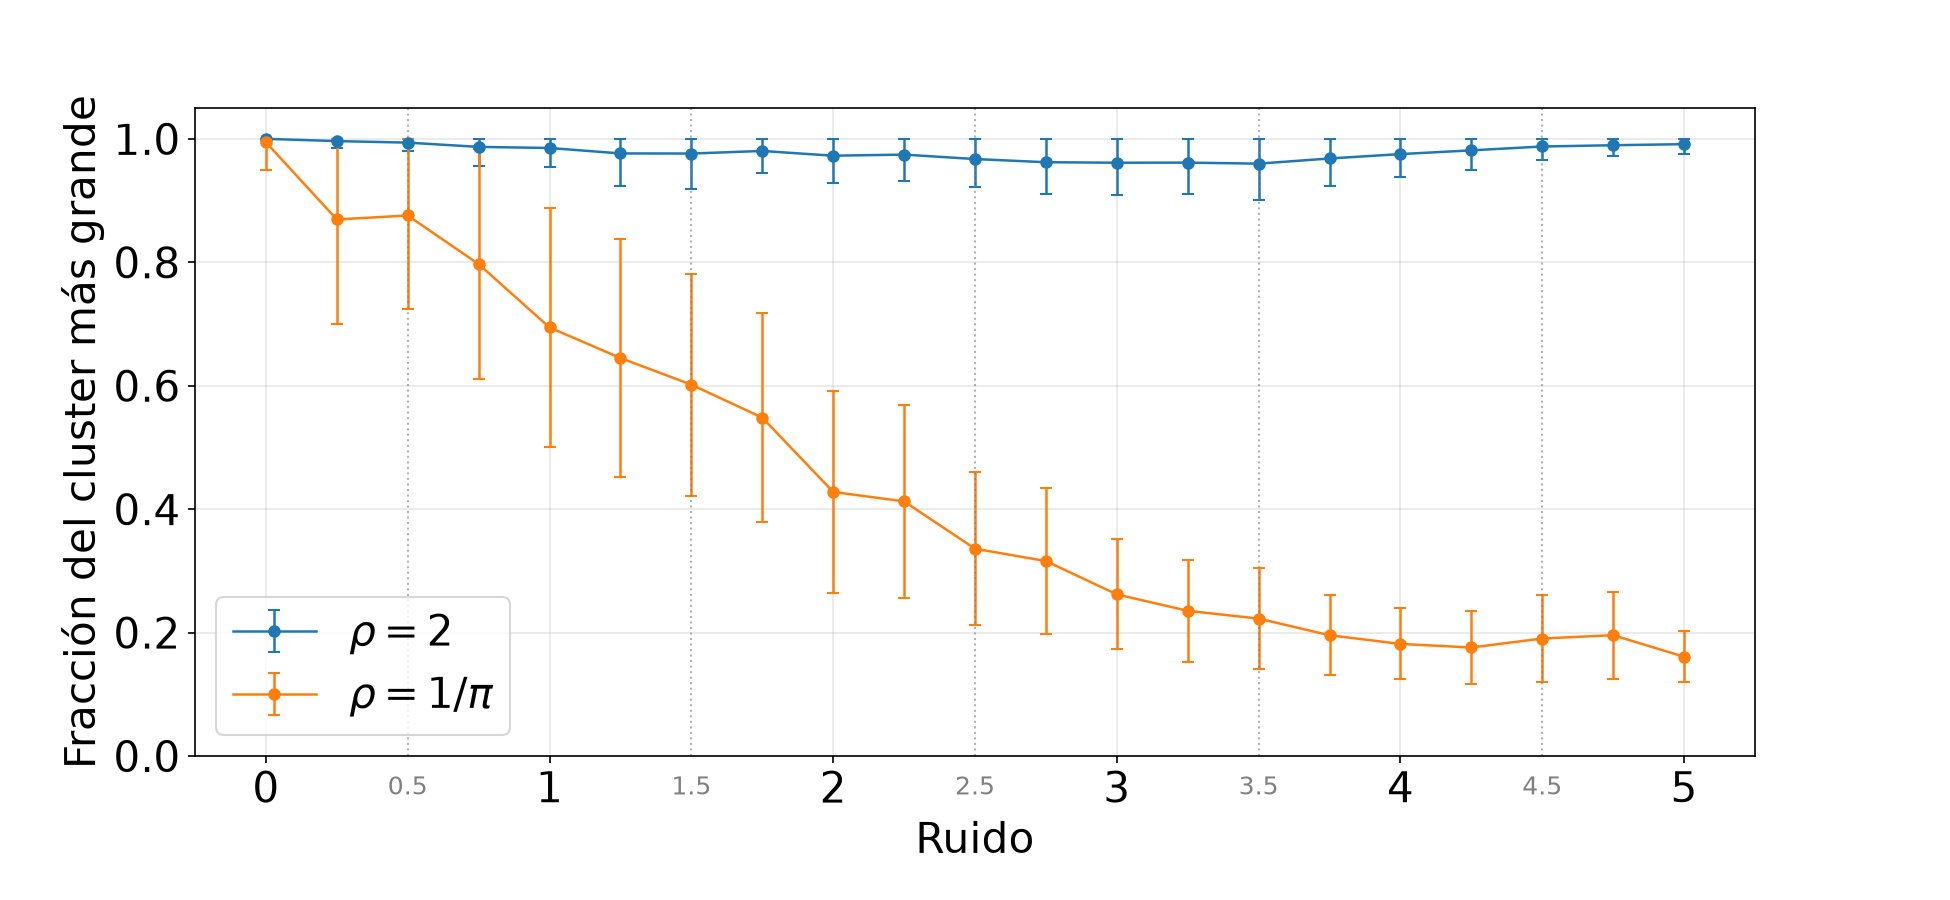
\includegraphics[width=0.75\textwidth]{entrega/d2/d2_standard_2_vs_low_30000.png}
  \caption{Fracción media del cluster más grande $\langle S \rangle \pm
    \sigma_S$ en función del ruido $\eta$, modelo estándar, para
    $\rho = 2$ y $\rho = 1/\pi$. $30\,000$ pasos.}
  \label{fig:d2-standard}
\end{figure}

\begin{center}
  \fbox{\parbox{0.9\textwidth}{\centering\small
  Animación -- modelo de votante, $\rho = 2$ y $1/\pi$, $\eta = 0$ y $1$:
  \href{https://youtu.be/XXXXX}{enlace pendiente}}}
\end{center}

La Fig.~\ref{fig:d2-voter} muestra el mismo análisis para el modelo de
votante: el mismo patrón que en el modelo estándar, $\rho = 2$
prácticamente constante cerca de $1$ y $\rho = 1/\pi$ decreciendo con
$\eta$, aunque con algunas oscilaciones locales adicionales.

\begin{figure}[h]
  \centering
  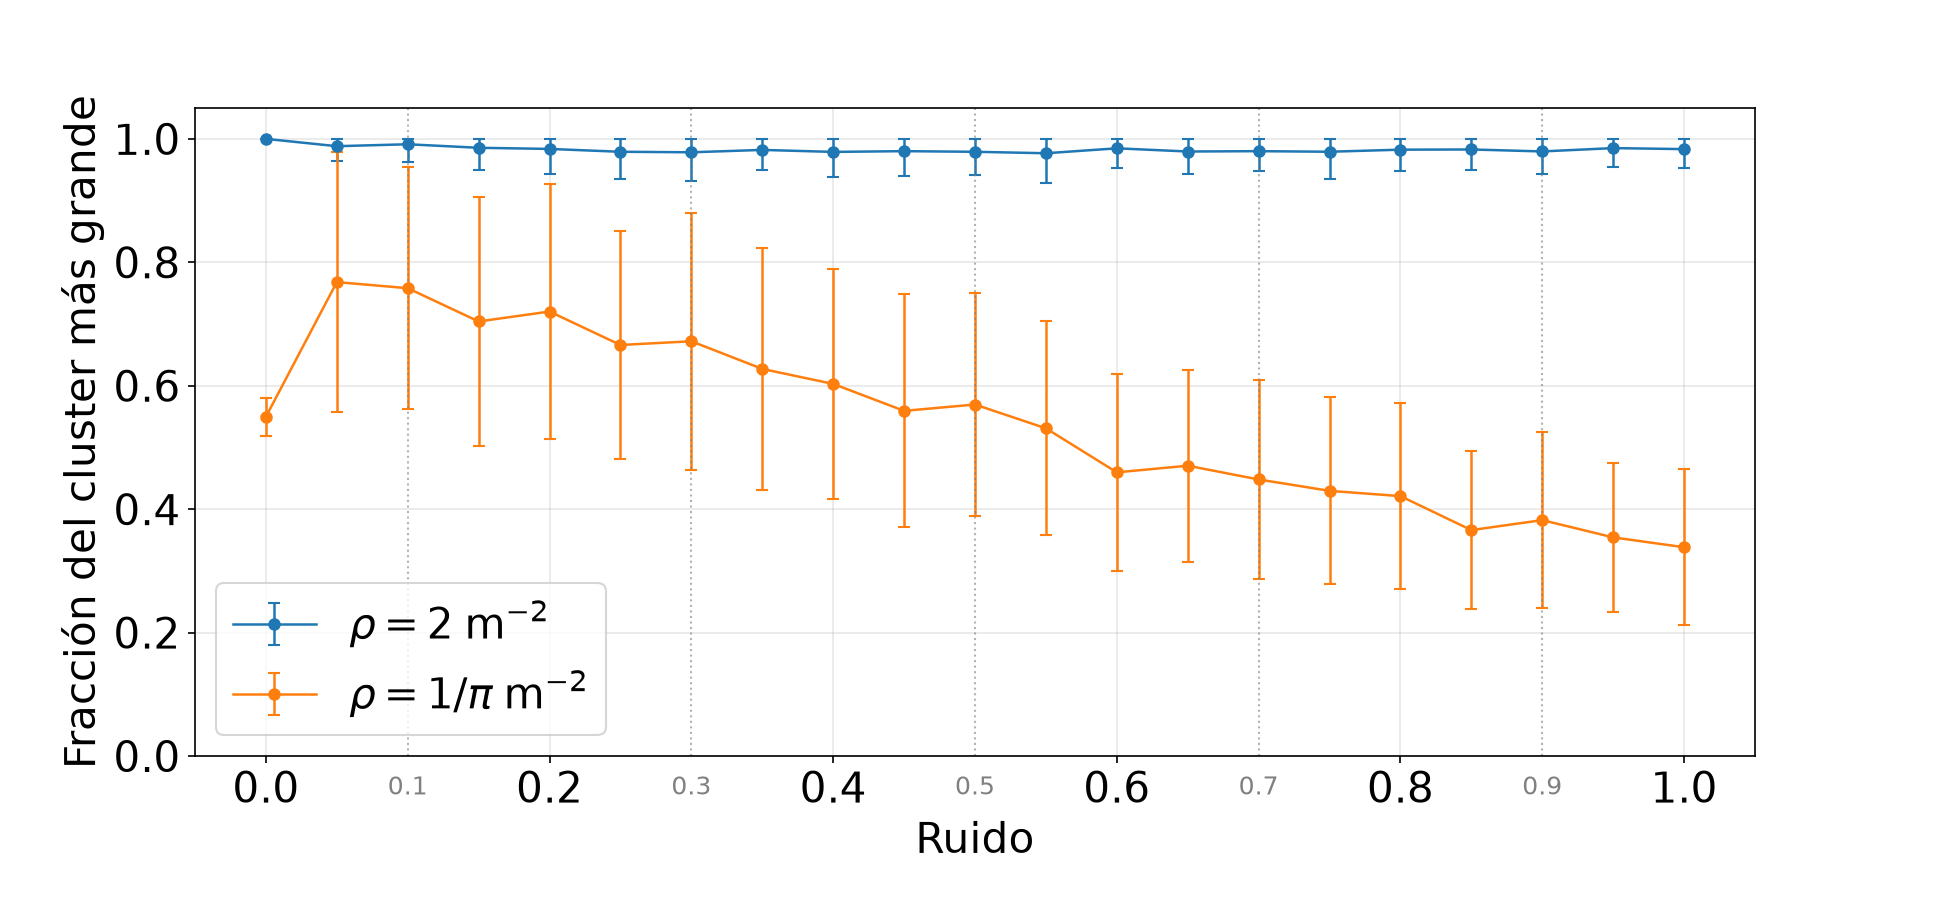
\includegraphics[width=0.75\textwidth]{entrega/d2/d2_voter_2_vs_low_30000.png}
  \caption{Fracción media del cluster más grande $\langle S \rangle \pm
    \sigma_S$ en función del ruido $\eta$, modelo de votante, para
    $\rho = 2$ y $\rho = 1/\pi$. $30\,000$ pasos.}
  \label{fig:d2-voter}
\end{figure}

\paragraph{Comparación estándar vs.\ votante ($\langle S \rangle$ vs.\ $\eta$)}

La comparación entre las Figs.~\ref{fig:d2-standard} y
\ref{fig:d2-voter} muestra que el comportamiento de $S$ frente al ruido es
cualitativamente el mismo en ambos modelos: la conectividad espacial está
gobernada principalmente por la densidad (geometría) cuando el sistema
está lejos del umbral de percolación, y sólo se vuelve sensible al ruido
$\eta$ cuando la densidad es marginal. Esto es consistente con que $S$, a
diferencia de $v_a$, no depende directamente de la regla de actualización
angular (Ec.~\eqref{eq:vicsek} o \eqref{eq:voter}) sino de las posiciones,
que en ambos modelos se actualizan de la misma forma
(Ec.~\eqref{eq:posicion}).

\subsection{Polarización vs. componente gigante}

Esta sección relaciona directamente los dos observables estudiados, $v_a$ y
$S$, para poner a prueba si el orden orientacional y la conectividad
espacial están correlacionados o son independientes entre sí. Para cada
modelo se graficó $\langle v_a \rangle$ en función de $\langle S \rangle$
(con barra de error en ambos ejes) para un conjunto de valores
representativos de $\eta$ y cuatro densidades: dos altas ($\rho = 2, 8$) y
dos bajas ($\rho = 1/\pi,\ 1/(3\pi)$). Los valores de $\eta$ usados son
$\{0, 1, 2, 5\}$ para el modelo estándar y $\{0.05, 0.4, 1\}$ para el
modelo de votante, cubriendo en cada caso desde el régimen ordenado hasta
el desordenado.

\begin{center}
  \fbox{\parbox{0.9\textwidth}{\centering\small
  Animación -- modelo estándar, $\rho = 1/(3\pi),\ 1/\pi,\ 2,\ 8$,
  $\eta = 0$ y $5$: \href{https://youtu.be/XXXXX}{enlace pendiente}}}
\end{center}

La Fig.~\ref{fig:e-standard} muestra el resultado para el modelo estándar.
Para las densidades altas ($\rho = 2$ y $\rho = 8$), los puntos se ubican
prácticamente sobre la recta vertical $S \approx 1$ para todo el rango de
$v_a$: como se vio en la Sección~\ref{sec:resultados}, a esas densidades el
sistema está muy por encima del umbral de percolación, así que $S$ no
depende del nivel de orden ni del ruido. Para las densidades bajas
($\rho = 1/\pi$ y $\rho = 1/(3\pi)$), en cambio, los puntos siguen una
tendencia creciente y aproximadamente monótona: a menor $v_a$ (mayor
ruido) le corresponde un $S$ menor, y ambos observables crecen juntos hasta
converger cerca de $(1,1)$ para $\eta$ chico. Esto confirma que $v_a$ y $S$
sólo están acoplados cuando la densidad es marginal respecto del umbral de
percolación; lejos de ese umbral, la conectividad se desacopla del orden
orientacional y queda gobernada únicamente por la geometría.

\begin{figure}[h]
  \centering
  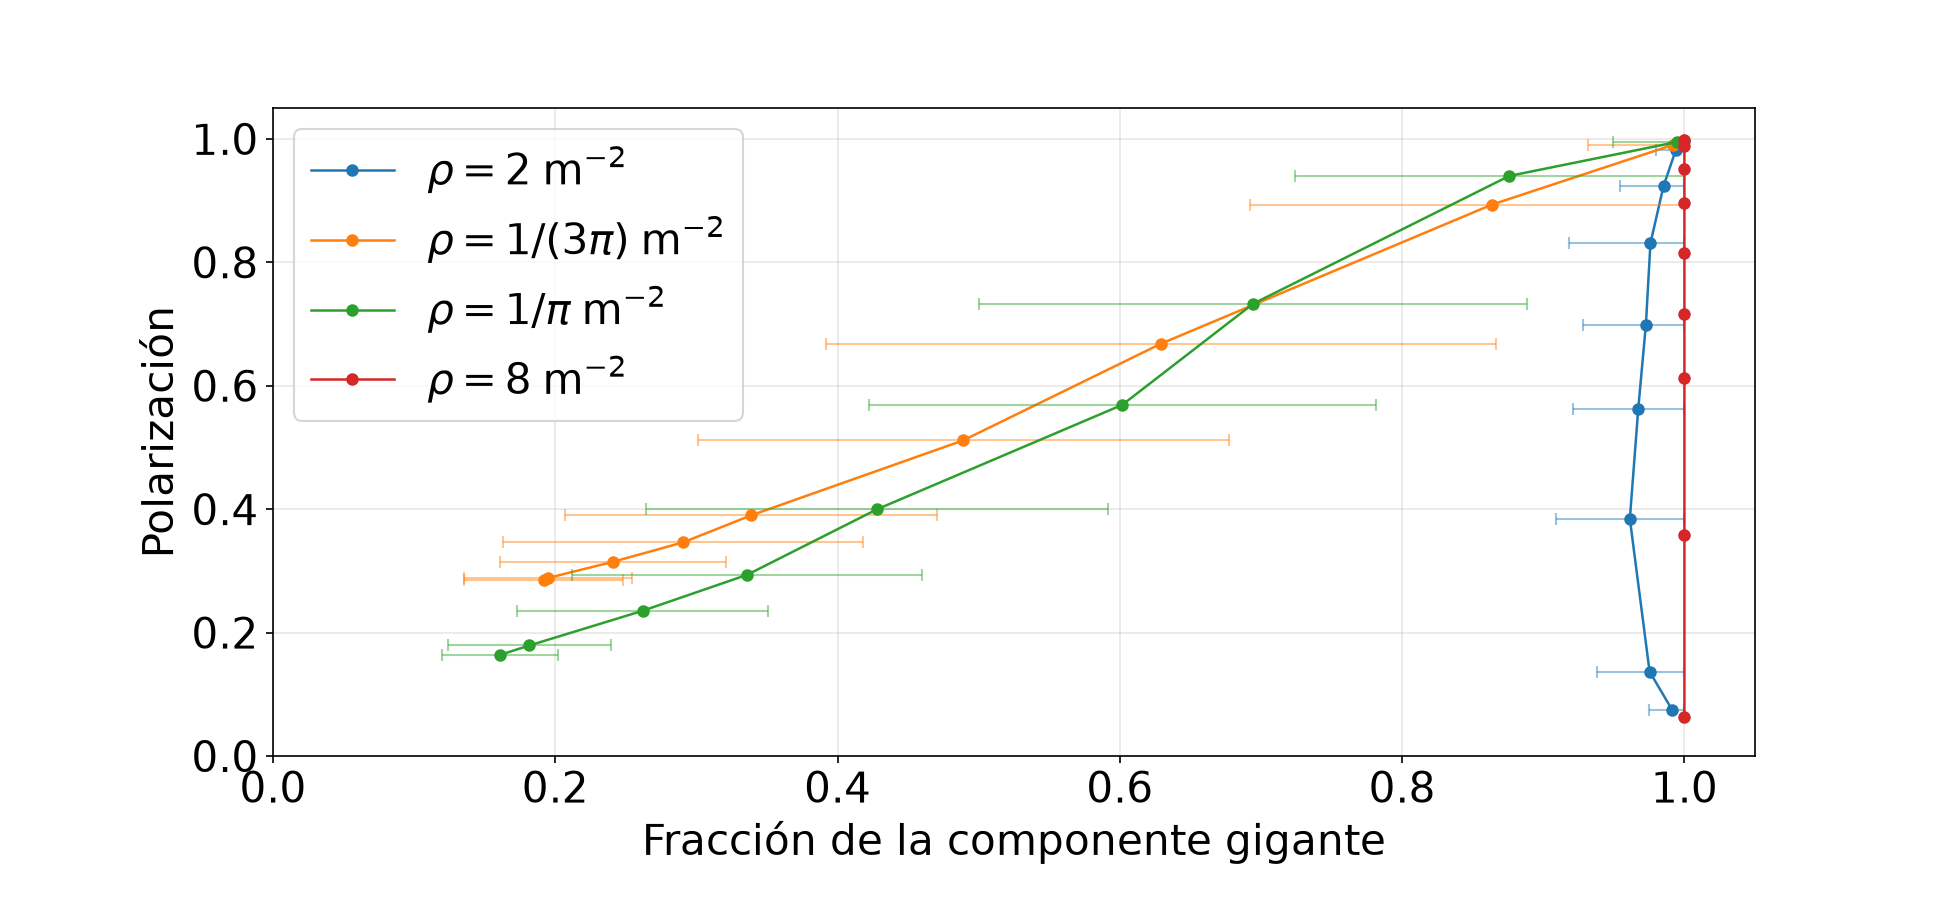
\includegraphics[width=0.75\textwidth]{entrega/e/e_standard_4dens_30000.png}
  \caption{Polarización media $\langle v_a \rangle$ en función de la
    fracción media del cluster más grande $\langle S \rangle$ (barras de
    error en ambos ejes), modelo estándar, para
    $\rho = 2,\ 8,\ 1/\pi,\ 1/(3\pi)$ y $\eta \in \{0, 1, 2, 5\}$.
    $30\,000$ pasos.}
  \label{fig:e-standard}
\end{figure}

\begin{center}
  \fbox{\parbox{0.9\textwidth}{\centering\small
  Animación -- modelo de votante, $\rho = 1/(3\pi),\ 1/\pi,\ 2,\ 8$,
  $\eta = 0.05$ y $1$: \href{https://youtu.be/XXXXX}{enlace pendiente}}}
\end{center}

La Fig.~\ref{fig:e-voter} muestra el mismo análisis para el modelo de
votante. El patrón general es el mismo -- densidades altas sobre la recta
$S \approx 1$, densidades bajas con $v_a$ y $S$ creciendo juntos -- pero la
relación entre ambos observables a densidad baja es menos suave que en el
modelo estándar: los puntos tienden a agruparse en dos regiones, una de
$\eta$ alto con $v_a$ y $S$ bajos ($\approx 0.3$--$0.4$) y otra de $\eta$
bajo con ambos altos ($\gtrsim 0.8$), con pocos puntos intermedios. Esto es
consistente con lo observado en la Sección~\ref{sec:resultados}: el modelo
de votante pierde el orden de forma más abrupta que el estándar en función
de $\eta$, y esa transición más abrupta en $v_a$ se traduce también en un
salto más marcado en $S$ para las densidades bajas.

\begin{figure}[h]
  \centering
  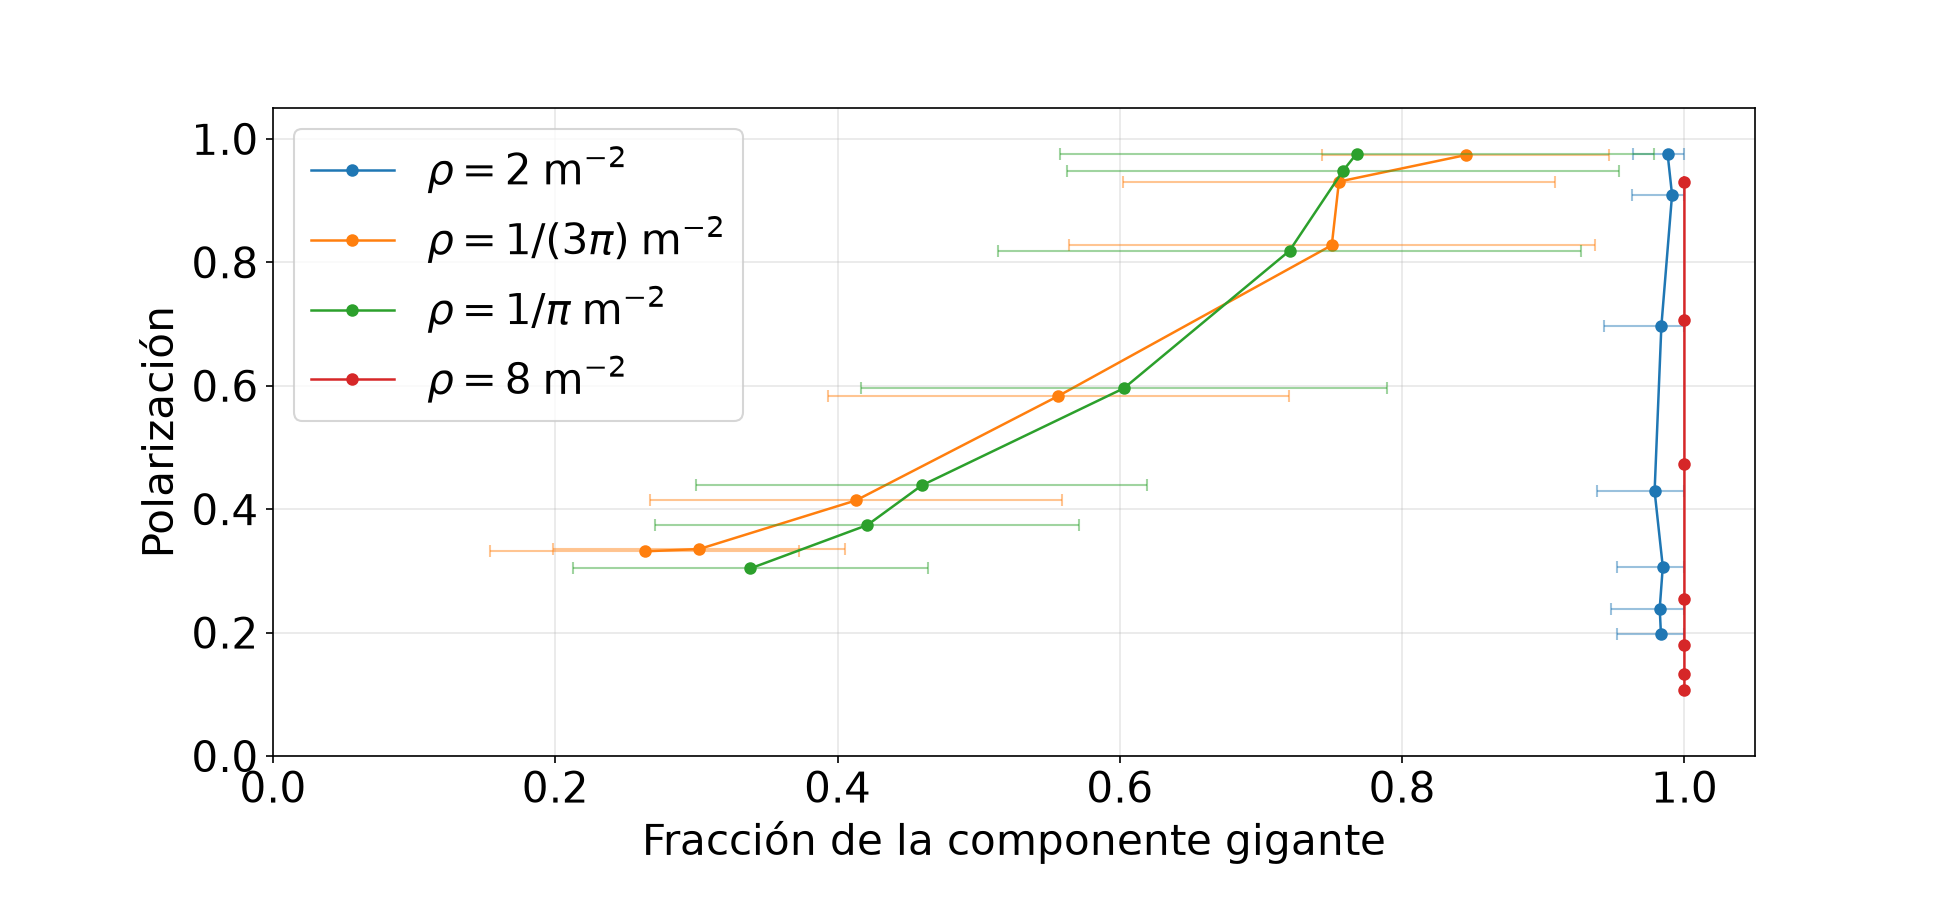
\includegraphics[width=0.75\textwidth]{entrega/e/e_voter_4dens_30000.png}
  \caption{Polarización media $\langle v_a \rangle$ en función de la
    fracción media del cluster más grande $\langle S \rangle$ (barras de
    error en ambos ejes), modelo de votante, para
    $\rho = 2,\ 8,\ 1/\pi,\ 1/(3\pi)$ y $\eta \in \{0.05, 0.4, 1\}$.
    $30\,000$ pasos.}
  \label{fig:e-voter}
\end{figure}

\paragraph{Comparación estándar vs.\ votante}

La comparación entre las
Figs.~\ref{fig:e-standard} y \ref{fig:e-voter} muestra que, en ambos
modelos, $v_a$ y $S$ están correlacionados
únicamente cuando la densidad es marginal respecto de la percolación
geométrica ($\rho = 1/\pi$, $1/(3\pi)$); a densidad alta ($\rho = 2$, $8$)
$S$ se satura en $1$ independientemente del orden orientacional. La
diferencia entre modelos, igual que en las secciones anteriores, es de
forma más que de fondo: la transición más abrupta del votante en $v_a$
también acelera el crecimiento de $S$ con el orden a densidad baja.

\section{Desempeño del método de las celdas (CIM)}
\label{sec:desempeno}

Además del comportamiento físico caracterizado en la
Sección~\ref{sec:resultados}, se evaluó el costo computacional del método
usado para la búsqueda de vecinos, ya que este cálculo se repite en cada
paso de tiempo y domina el costo total de la simulación. Se compararon los
tiempos de ejecución de un pase completo del CIM (armado de la grilla y
consulta de vecinos de todas las partículas, sobre una configuración
estática, sin evolucionar la simulación) entre la
implementación de este TP y una versión del algoritmo del TP1 portada a
C++, ambas con arreglos planos reutilizados entre corridas para no medir
costos de asignación de memoria. La medición sigue el mismo esquema de
lotes usado en el TP1: lotes de $100$ corridas por muestra, con $3000$
muestras para $N \leq 200$ y $30$ para $N > 200$.

La Fig.~\ref{fig:g-cim} muestra el tiempo medio (con su desvío) en función
del número de partículas $N$, en escala doble logarítmica. Para $N$ chico
($N \lesssim 35$) el CIM de este TP es más rápido que el del TP1, pero a
partir de ese cruce el algoritmo del TP1 resulta más eficiente, con una
diferencia que crece con $N$. La causa es algorítmica: el CIM del TP1
recorre sólo $4$ direcciones vecinas más la celda propia y evalúa cada par
de partículas una única vez, mientras que el CIM de este TP consulta las
$9$ celdas vecinas por partícula, evaluando cada par dos veces (una desde
cada partícula). Ambos algoritmos son $O(N)$ para densidad fija, por lo que
el cruce refleja una diferencia de constante multiplicativa y no de orden
de complejidad.

\begin{figure}[h]
  \centering
  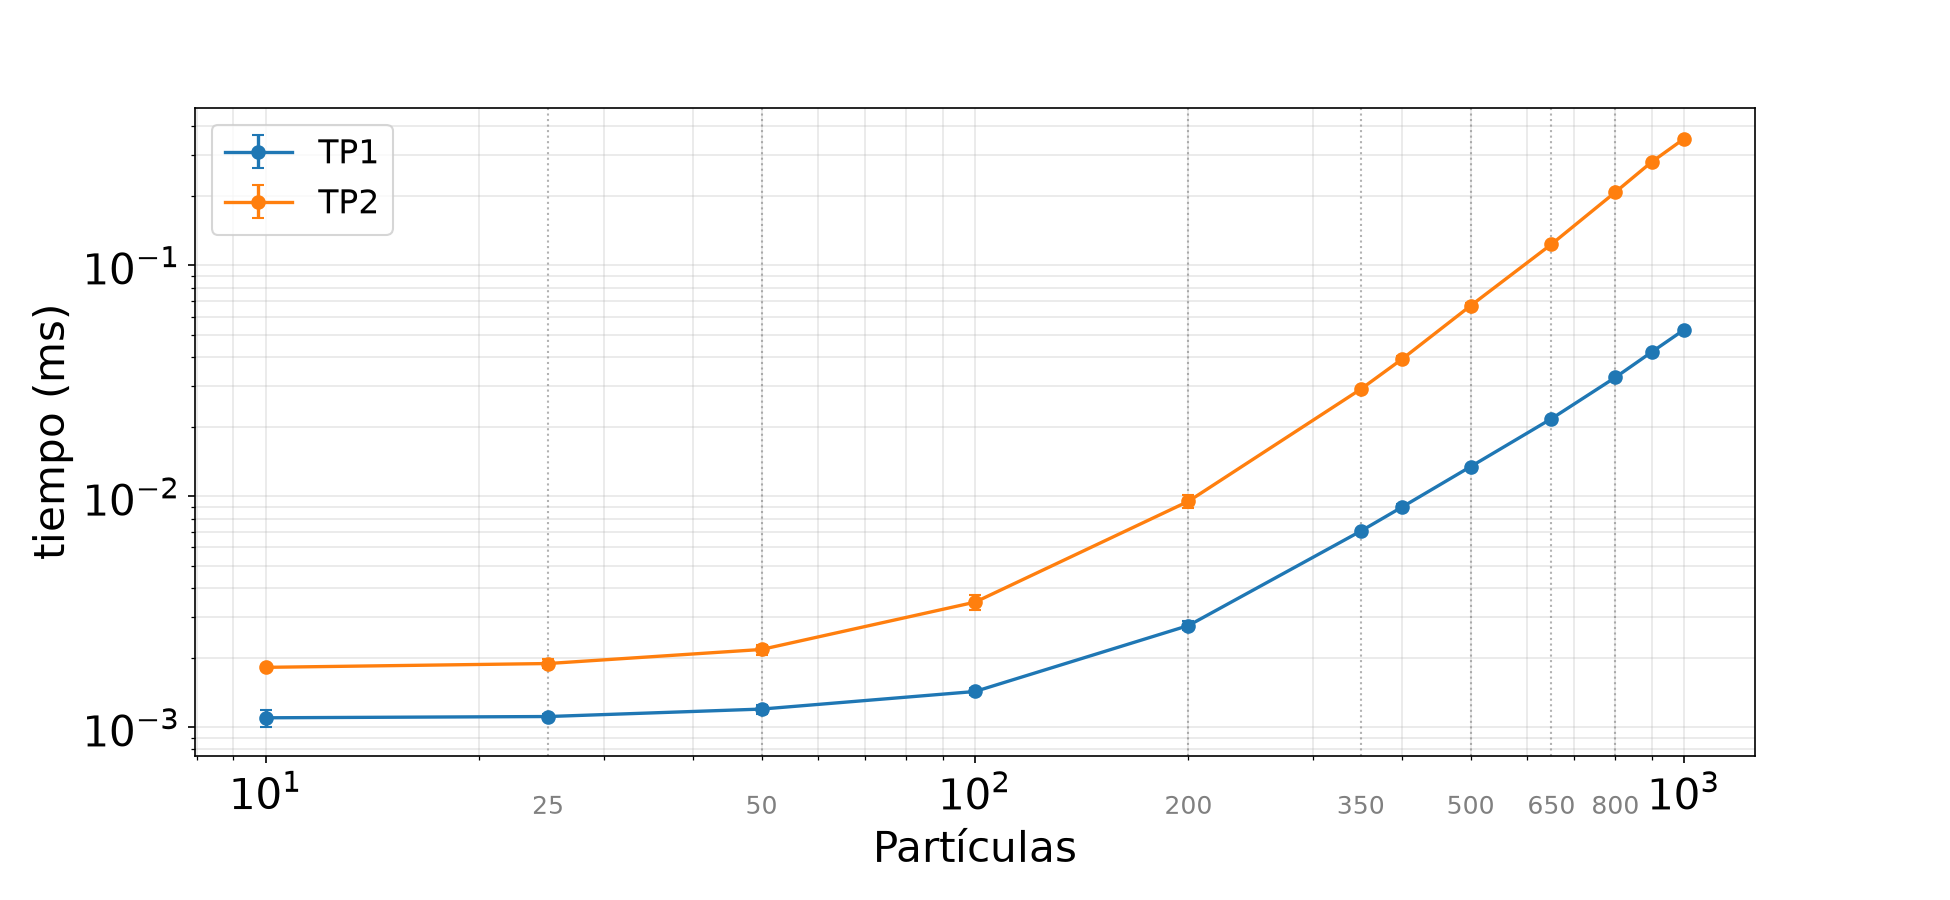
\includegraphics[width=0.75\textwidth]{entrega/g/g_cim_vs_tp1.png}
  \caption{Tiempo de un pase completo del CIM en función del número de
    partículas $N$, comparando la implementación de este TP (TP2) con el
    algoritmo del TP1 portado a C++. Escala doble logarítmica.}
  \label{fig:g-cim}
\end{figure}

\section{Conclusiones}

\begin{center}
  \fbox{\parbox{0.9\textwidth}{\centering\small
  [Conclusiones pendientes -- a completar por el grupo.]}}
\end{center}

\begin{thebibliography}{9}

\bibitem{vicsek1995}
T. Vicsek, A. Czirók, E. Ben-Jacob, I. Cohen, O. Shochet,
``Novel type of phase transition in a system of self-driven particles,''
\emph{Physical Review Letters}, vol.\ 75, no.\ 6, pp.\ 1226--1229 (1995).

\bibitem{loscar2021}
E. S. Loscar, G. Baglietto, F. Vazquez,
``Noisy multistate voter model for flocking in finite dimensions,''
\emph{Physical Review E}, vol.\ 104, no.\ 3, 034111 (2021).

\end{thebibliography}

\end{document}
